\documentclass[en]{minipw} % wszystkie ustawienia szablonu są w minipw.cls; if in English, change [pl] to [en]
\allowdisplaybreaks
\usepackage{indentfirst}
\setlength{\parindent}{5mm} % wcięcie akapitowe 5mm, zarządzenie Rektora

\usepackage{algorithm}
\usepackage{mathtools}
\usepackage{amsmath}

\usepackage[noend]{algpseudocode}

\setcounter{MaxMatrixCols}{20}

% ------------ Ustawienia autora pracy ---------------

\setboolean{lady}{false} % kobiety wpisują true, mężczyźni - false

\title{Deformation of Soft Bodies on GPU} % nazwa pracy
\titleaux{Deformacje Ciał Odkształcalnych na GPU}
\type{magisters} % licencjat = licencjac, inżynier = inżyniers
\discipline{Informatyka} % kierunek
\specjal{Projektowanie Systemów CAD/CAM}
\author{Jakub Ciecierski}
\album{243260}
\supervisor{dr~inż. Joanna Porter-Sobieraj}
\konsultacje{prof. Dumbledore} % jeśli nie ma, trzeba zakomentować też w minipw.cls
\date{2018}
\klucze{Deformacje Ciał Odkształcalnych, Metoda Elementów Skończonych, Mechanika Ciał Stałych ,GPU, CUDA}
\keywords{Soft Body, Finite Element Method, Solid Mechanics, Real-Time, GPU, CUDA, Physics engine, Game physics, Simulation, Deformation}
% ----------------------------------------------------

\begin{document}
\sloppy

% Nowy układ pracy dyplomowej

% 1. Strona tytułowa - trzeba wydrukować z osobnego pliku


% 2. Streszczenia
% Streszczenie ma zawierać tytuł pracy i słowa kluczowe
% if in English, English abstract goes first


\setcounter{page}{1}

\begin{abstract}
This thesis provides an overview of real-time soft body deformation methods. The goal of this study is to design and implement numerical library solving the problem of physically correct soft body deformations. GPU accelerated Finite Element Method is used which solves the problem of solid mechanics for linear geometry and linear material properties. The library is integrated into existing open source game engine.

\end{abstract}

\begin{streszczenie}



\end{streszczenie}


% 2. Oświadczenie o autorstwie pracy - w innym pliku
\makestatement


% 4. Spis treści
\cleardoublepage
\tableofcontents

% 5. Treść

\cleardoublepage
\pagestyle{fancy}

\chapter*{Introduction}
With the growth of popularity in virtual reality hardware comes great responsibility for software engineers to provide realistic and detailed experiences. User wearing virtual reality headset such as Oculus Rift is closer to the virtual environment than ever before. She will expect full interaction with the environment around her. The object she will pick up can be seen from very close distance. This requirement pushes software and hardware engineers alike to the frontier of computer graphics to provide detailed and authentic experiences. However, the user will also expect the virtual object to behave in a physically correct way. Virtual reality controllers gives us a chance to grab and interact with objects using our own hands. We should expect a virtual object to deform when enough pressure is applied to it. Thus, it is our responsibility as engineers to develop physics engines suitable for such tasks.

Real-time soft body deformation simulations have many practical applications. It provides more realistic and thus more fun gaming experiences. Soft body simulation is extremely useful in educational applications such as real time virtual surgery tutorial. Real time virtual car crash testing can provide fast and extremely cheap way to analyse car deformation in case of accident.

Topic of this thesis is motivated by the ever increasing requirements of virtual environment users and by the rapid growth of hardware capabilities in a form of GPU computational power. This thesis provides an overview of current methods used in real-time soft body deformations. The goal is to design and implement numerical library that would solve the problem of soft body deformation in real-time. Moreover, the library should provide friendly interface which support easy integration into existing virtual reality engines(e.g. game engines). The author proposes an integration into open source engine of his own creation~\cite{ifx}.

The author chooses Finite Element Method(FEM) based simulation of soft bodies. It is the most physically correct method studied in this thesis. However, it comes with a price of expensive computations. FEM is used to solve the problem of solid mechanics with linear geometry and linear material properties. The linearity of the system enables us to work only with linear system of equations which can be computed much faster than the non-linear systems. However, the linear formulation is visibly pleasing only for small deformations. Linear tetrahedron finite element is chosen which is quite suitable for real time simulations. Implicit euler method is used for integrating the differential equations of the dynamic system.

Understanding FEM from theoretical point of view might seem daunting at first. However, the study of applied mechanics have been extremely active for over three decades. Zienkiewicz in~\cite{zienkiewicz1} and~\cite{zienkiewicz2} provides thorough explanation of FEM and its applications in solid mechanics. Kleiber and Kowalczyk~\cite{termo} familiarise the reader with the basics of tensor algebra, stress analysis and material properties. Lectures at University of Colorado~\cite{colorado_fem_lectures} guide the reader through linear FEM. Moreover, they provide example functions written in Mathematica that can be used to test implementation of custom FEM solver. Altair University~\cite{altair} shows practical applications of FEM aimed at material engineers.

Parker~\cite{parker} implements linear FEM solver that focuses on game environments settings. He designed an algorithm based on implicit time integration on the CPU side. Moreover, the solution contains a fracture mechanics which enables objects to be broken under certain stress threshold.
Faure et al. in~\cite{tensor-mass} provide alternative to classical FEM called Tensor-Mass approach. This approach computes the forces applied directly on the vertices. Faure et al. implements a GPU accelerated solver using the SOFA framework~\cite{sofa}.
Zhuang et al. were interested in non-linear FEM solver~\cite{global_deformation}. Experiments of their CPU implementation gave reasonable results thanks to the diagonalization of mass and damping matrices.

In chapter~\ref{chap:background} the thesis starts with a background study of current methods of solving the problem of soft body deformations. It familiarises reader with numerical integration of differentiable equations and provides an overview of currently commercially available physics engines.
Further in chapters~\ref{chap:solid_mechanics1} and~\ref{chap:solid_mechanics2} detailed explanation of solid mechanics and finite element method is provided. Here, the reader is set on a journey to transform linear partial differential equations(PDE) to linear system of algebraic equations. Then in chapter~\ref{chap:system_linear} method of solving the system of linear equations is described in a form of  Conjugate Gradient.
One of the greatest difficulties in FEM solver is creating an 3D computation mesh satisfying our problem domain. This thesis is out of scope of detailed explanations of tetrahedralization process, however a short overview is provided in chapter~\ref{chap:Tetrahedralization}.
Chapter~\ref{chap:Implementation} shows the implementation of the library and its integration into open source game engine.
The thesis ends with chapters~\ref{chap:tests} and~\ref{chap:Conclusions} where the author tests and provides conclusions of created algorithm.
% ---------------------------------------------------

\chapter{Background}
\label{chap:background}

\section{Mass Spring}
\subsection{Formulation}
The simplest method to simulate soft body deformation is Mass Spring System.
Such a system includes a set of $N$ particles with masses $m_i$, positions $x_i$ and velocities $v_i$, where $i \in 1...N$. The particles are connected by a set of springs $S$. A single spring $s \in S$ consists of $s = (i, j, l_0, k_s, k_d)$, where $i$ and $j$ are the indices of connected particles, $l_0$ is the rest length, $k_s$ is the spring stiffness and $k_d$ is the damping coefficient. To calculate the forces acting on particles $i$ and $j$, we use the following formula:

\begin{equation}
f_{i}^{S} = f^{S}(x_i, x_j) = k_s \dfrac{x_j - x_i}{|x_j - x_i|}(|x_j - x_i| - l_0)
\end{equation}
\begin{equation}
f_{j}^{S} = f^{S}(x_j, x_i) = -f^{S}(x_i, x_j)
\end{equation}

It is easy to see that the forces conserve momentum, since ($f_i + f_j = 0$)

We apply damping by computing the damping forces:

\begin{equation}
f_{i}^{D} = f^{D}(x_i, v_i, x_j, v_j) = k_d (v_j - v_i) \dfrac{x_j - x_i}{|x_j - x_i|}
\end{equation}

\begin{equation}
f_{j}^{D} = f^{D}(x_j, v_j, x_i, v_i) = -f_{i}^{D}
\end{equation}

Combining two forces we get the final spring force

\begin{equation}
f(x_i, v_i, x_j, v_j) = f^{S}(x_i, x_j) + f^{D}(x_i, v_i, x_j, v_j)
\end{equation}

\subsection{Simulation}
In order to simulate the mass spring system, we use the Newton's second law of motion,

\begin{equation}
f = m \ddot{x}
\end{equation}

where $f$ is the force, $m$ is the mass and $\ddot{x}$ is the acceleration or the second derivative of position with respect to time. By transforming the equation to solve for acceleration, we get a second order ordinary differential equation(ODE):
\begin{equation}
\ddot{x} = \dfrac{f}{m}
\end{equation}

In order to solve it, we can split this equation into two first order ODEs

\begin{equation}
\label{eq:ode_v} 
\dot{v} = \dfrac{f}{m}
\end{equation}
\begin{equation}
\label{eq:ode_x} 
\dot{x} = v
\end{equation}

Analytically, these can be solved by definite integrals:

\begin{equation}
\label{eq:ode_anal1}
v(t) = v_0 \int_{t_0}^{t} \dfrac{f(t)}{m} dt
\end{equation}

\begin{equation}
\label{eq:ode_anal2}
x(t) = x_0 \int_{t_0}^{t}v(t) dt
\end{equation}

where $v_0 = v(t_0)$ and $x_0 = x(t_0)$ are the initial conditions.

\subsection{Numerical Integration}

\subsubsection{Explicit Euler Integration}

One of the most basic numerical integration of ODE is explicit Euler integration scheme. The scheme approximates the derivatives using finite differences:

\begin{equation}
\dot{v} = \dfrac{v^{t+1} - v^{t}}{\Delta t}
\end{equation}
\begin{equation}
\dot{x} = \dfrac{x^{t+1} - x^{t}}{\Delta t}
\end{equation}

where $\Delta t$ is a discrete time step and $t$ is the index of the simulation iteration. By substituting these equations into Eq.~\ref{eq:ode_v} and Eq.~\ref{eq:ode_x}, we get get the explicit Euler integration method:
\begin{equation}
\label{eq:explicit_euler_ode_v}
v^{t+1} = v^{t} + \Delta t \dfrac{f(x^{t}, v^{t})}{m}
\end{equation}
\begin{equation}
\label{eq:explicit_euler_ode_x}
x^{t+1} = x^{t} + \Delta t v^{t+1}
\end{equation}

The term 'explicit' comes from the fact that information of the next time step can be directly computed using the information at the current time step.

The entire simulation can be summed with the following algorithm:

\begin{algorithm}
\caption{Mass Spring Simulation}\label{euclid}
\begin{algorithmic}[1]
\Procedure{Simulation}{}
\While{true}
\For {all particles $i$}
\State $f_i = f^{g} + f_{i}^{coll} + \sum_{j, (i,j) \in S} f(x_i, v_i, x_j, v_j)$
\EndFor

\For {all particles $i$}
\State $v_{i} = v_{i} + \Delta t \dfrac{f_i}{m_i} $
\State $x_{i} = x_{i} + \Delta t v_i $
\EndFor

\EndWhile

\EndProcedure
\end{algorithmic}
\end{algorithm}

$f^{g}$ is the gravity force and $f^{coll}$ collision forces.

A known drawback for explicit Euler integration is the fact that it requires small time steps to remain stable. This problem occurs because explicit Euler does not account for the near future and it assumes that the force is constant during the entire time step. Let us assume a system of two particles connected with a spring. Assume the following configuration: the spring is stretched and the two particles start moving towards each other. If we take a large time step to compute the next configuration, the particles might pass the equilibrium configuration, which in theory means that the force should change its sign during that time step. Sadly, since the force is constant throughout the entire time step, the sign change of the force is not accounted for. This might lead to particles overshooting and gaining energy which in turn leads to a so called simulation explosion.
Other numerical integration methods exist that are more accurate. Among the most popular are the second and fourth order Runge-Kutta integrators. These schemes compute forces multiple times during a single time step, which might reduce the effect of the problem mentioned above.

\subsubsection{Runge-Kutta Integration}
The second order Runge-Kutta integrator has a different method of numerically solving ODEs. The approximation of explicit Euler Eq.~\ref{eq:explicit_euler_ode_v} and Eq.~\ref{eq:explicit_euler_ode_x} are instead computed by the formulas:


\begin{equation}
\begin{aligned}
a_1 = v^t
\\
a_2 = \dfrac{f(x^t, v^t)}{m}
\\
b_1 = v^t + \dfrac{\Delta t}{2} a_2
\\
b_2 = \dfrac{f(x^t + \dfrac{\Delta t}{2} a_1, v^t + \dfrac{\Delta t}{2} a_2)}{m}
\\
x^{t+1} = x^{t} + \Delta t b_1
\\
v^{t+1} = v^{t} + \Delta t b_2
\end{aligned}
\end{equation}

It is easy to see that the forces are computed twice during one time step. This makes the second order Runge-Kutta integrator more accurate compared to the simple first order explicit Euler method.

One of the most popular methods of integrating ODE is a forth order Runge-Kutta integrator. It extends the the second order Runge-Kutta by computing the force four times during a single time step. Making it even more accurate. The accuracy obviously comes with longer computations.

\subsubsection{Implicit Euler}
Another way to improve stability is to use implicit integrator. Among the most popular is the implicit Euler method. As opposed to explicit integrators, the implicit is more physically correct.
\begin{equation}
\label{eq:implicit_euler_ode_v}
\begin{aligned}
v^{t+1} = v^{t} + \Delta t \dfrac{f(x^{t+1})}{m}
\\
x^{t+1} = x^{t} + \Delta t v^{t+1}
\end{aligned}
\end{equation}
First difference lies in the force function $f$. Now it only depends on the position. In another words, the force does not include friction. It is said that implicit integration introduces enough numerical damping to accommodate for physical damping. However, if needed, the friction force can be added in the explicit step after the implicit solve. The most important change, is the fact that the force $f$ depends now on the position of next step $x^{t+1}$. Thus, it is no longer possible to explicitly compute the two equations. Instead we now deal with a algebraic system, with unknowns being $x^{t+1}$ and $v^{t+1}$.

In order to compute these equation we must first construct the algebraic system. The position, velocities and forces are concatenated into vectors:
\begin{equation}
\begin{aligned}
x = [x_1, x_2, ..., x_n]
\\
v = [v_1, v_2, ..., v_n]
\\
f(x) = [f_1(x_1,..., x_n), ..., f_n(x_1,..., x_n)]
\end{aligned}
\end{equation}
Further, we construct a mass matrix $M \in \mathbb{R}^{3N \times 3N}$ which is diagonal with values $m_1, m_1, m_1, ..., m_N, m_N, m_N$ on the diagonal.

\begin{equation}
\label{eq:implicit_mass_ode_v}
M v^{t+1} = M v^{t} + \Delta t f(x_{t+1})
\end{equation}
\begin{equation}
\label{eq:implicit_mass_ode_x}
x^{t+1} = x + \Delta t v^{t+1}
\end{equation}

Substituting Eq.~\ref{eq:implicit_mass_ode_x} into Eq.~\ref{eq:implicit_mass_ode_v}, results in single system of algebraic equations:

\begin{equation}
M v^{t+1} = M v^{t} + \Delta t f(x + \Delta t v^{t+1})
\end{equation}

We solve this system for $v^{t+1}$.

Example implementation of mass spring system can found in open source software created by the author of this thesis in~\cite{JC-MassSpring}. 

\subsubsection{Conclusions}
Mass spring systems are easy to implement and for many applications give good enough results(e.g. computer games). However, relatively expensive ODE integrators have to be used in order to keep the simulation stable. Moreover, modelling physically correct materials can be a complicated task, since the parameters of the system hardly reflect reality.

\section{Position Based Dynamics}
As the name suggests, Position Based Dynamics(PBD) omits integrating over velocity and works directly on positions. The biggest advantage over mass spring system is avoidance of overshooting problem during integration step.
\subsection{Formulation}
The system of PBD includes a set of $N$ particles and a set of $M$ constraints. Each particle $i$ has three attributes: 
\begin{enumerate}
\item mass $m_i$
\item position $x_i$
\item velocity $v_i$
\end{enumerate}

Each constraint $j$ has five attributes:

\begin{enumerate}
\item Cardinality - $n_j$
\item Scalar constraint function - $C_j : \mathbb{R}^{3n_j} \rightarrow \mathbb{R}$
\item Set of indices - $\{i_1, ..., i_{n_{j}}\}, i_k \in [1, ..., N]$
\item Stiffness parameter - $k_j \in [0 ... 1]$
\item Type - \textit{unilateral} or \textit{bilateral}
\end{enumerate}

It is said that bilateral constraint $j$ is satisfied if $C_j(x_{i_{1}}, ..., x_{i_{n_{j}}}) = 0$ or if the case of unilateral $C_j(x_{i_{1}}, ..., x_{i_{n_{j}}}) \geq 0$. The strength of the constraint is defined by the stiffness parameter $k_j$.

Given initial conditions for positions and velocities the simulation proceeds as follows:


\begin{algorithm}
\caption{Particle Based Dynamics}\label{euclid}
\begin{algorithmic}[1]
\Procedure{Simulation}{}

\While{true}
\label{alg:pbd:main_loop}

\For {all particles $i$}
\label{alg:pdb:explicit_for}

\State $v_{i} = v_{i} + \Delta t \dfrac{f_i}{m_i}$
\label{alg:pdb:explicit_v}

\State $p_{i} = x_{i} + \Delta t v_i$
\label{alg:pdb:explicit_p}

\State $generateCollisionContraints(x_i, p_i)$
\label{alg:pdb:generate_collision_contraints}

\EndFor

\While{iteratively}
\label{alg:pdb:iter_while}

\State $projectContraints(C_1, ..., C_{M + M_{ext}}, p_1, ..., p_N)$
\label{alg:pdb:project_contraints}

\EndWhile

\For {all particles $i$}
\State $v_{i} = \dfrac{(p_i - x_i)}{\Delta t} $
\label{alg:pdb:implicit_v}

\State $x_{i} = p_{i}$
\label{alg:pdb:implicit_x}

\EndFor

\EndWhile

\EndProcedure
\end{algorithmic}
\end{algorithm}

The lines~\ref{alg:pdb:explicit_v} and~\ref{alg:pdb:explicit_p} compute explicit Euler integration on velocities and positions. However, output positions $p_i$ are only used as predictions. 
The line ~\ref{alg:pdb:generate_collision_contraints} generates external constrain such as collisions. The original and predicted positions $x_i$, $p_i$ can be used in this step in order to perform continuous collision detection.
The simulation then computes line~\ref{alg:pdb:project_contraints} which iteratively corrects the predicted positions such that they satisfy the $M_{ext}$ external and $M$ internal constraints.
Finally, the corrected positions $p_i$ are used to compute velocities and positions. For more information about PDB the reader is encouraged to read~\cite{physics_notes}.
PDB has found its usage in nvidia's Flex library~\cite{flex}.

\section{Finite Element Method}
Mass spring systems can not simulate physically correct volumetric effects. Moreover, it highly depends on the structure of the spring mesh. Finally, the parameters in previous soft body dynamics systems have no physical intuition. Thus it is hard to create different physical materials. All these limitations can be suppressed by the Finite Element Method. Soft body dynamics based on FEM are not yet common in the real time environment. One of the most successful usages of FEM in real time simulation were done by~\cite{parker}. The authors were able to integrate their FEM solver in the game called Star Wars: The Force Unleashed. The details on FEM formulation will follow in next chapters.

% ---------------------------------------------------
\chapter{Solid Mechanics - Part 1}
\label{chap:solid_mechanics1}

\section{Formulation}
\subsection{Displacement}
Displacement field $u(x)$ is a first order tensor, or a three dimensional vector. It defines the translation of body object. For clarity we will often omit the input position vector $x$ and use the simplified tensor notation $u_i$

\subsection{Strain}
Strain tensor is the measure of elongation of the material. It is defined as second order symmetric tensor $\epsilon$.
\begin{equation}
\begin{aligned}
\epsilon =
\begin{bmatrix}
\epsilon_{11} & \epsilon_{12} & \epsilon_{13} \\
\epsilon_{12} & \epsilon_{22} & \epsilon_{23} \\
\epsilon_{13} & \epsilon_{23} & \epsilon_{33} \\
\end{bmatrix}
\end{aligned}
\end{equation}
Strain tensor can be computed in many ways. The linear version $\epsilon_C$ called Cauchy's linear strain tensor is defined by:
\begin{equation}
\begin{aligned}
\epsilon_C = \dfrac{1}{2}(\Delta u + (\Delta u)^{T})
\end{aligned}
\end{equation}
where the gradient of displacement $u$ is defined:
\begin{equation}
\begin{aligned}
\Delta u =
\begin{bmatrix}
u_{1,1} & u_{1,2} & u_{1,3} \\
u_{2,1} & u_{2,2} & u_{2,3} \\
u_{3,1} & u_{2,2} & u_{3,3} \\
\end{bmatrix}
\end{aligned}
\end{equation}

In tensor notation the spatial derivative is denoted by: $u_{1,1} = \dfrac{\partial u_1}{\partial x_1}$.

\subsection{Stress}
Let us defined traction force vector $t$ as a density of forces $f$ acting on an area $A$ of a certain body point:
\begin{equation}
\begin{aligned}
t = \dfrac{df}{dA}
\end{aligned}
\end{equation}
Traction force acts with some magnitude along the normal vector $n$ to the snippet element with area $A$. The magnitude is defined by second order, symmetric stress tensor $\sigma$.
\begin{equation}
\begin{aligned}
t = \sigma n
\end{aligned}
\end{equation}

Stress tensor is defined by:
\begin{equation}
\begin{aligned}
\sigma =
\begin{bmatrix}
\sigma_{11} & \sigma_{12} & \sigma_{13} \\
\sigma_{12} & \sigma_{22} & \sigma_{23} \\
\sigma_{13} & \sigma_{23} & \sigma_{33} \\
\end{bmatrix}
\end{aligned}
\end{equation}

\subsection{Constitutive Laws}
We defined three dimensional Hooke's law which defines a linear relation between stress and strain
\begin{equation}
\begin{aligned}
\sigma_{ij} = C_{ijkl}\epsilon_{kl}
\end{aligned}
\end{equation}

The fourth order tensor $C$ is called a spring stiffness tensor. Tensor $C$ does not depend on $x$ and is composed of only constant material parameters. In case of isotropic materials(material that behave the same in all directions of motion) the Hooke's law can be defined by the system:
\begin{equation}
\begin{aligned}
\begin{bmatrix}
\sigma_{11} \\
\sigma_{22} \\
\sigma_{33} \\
\sigma_{12} \\
\sigma_{23} \\
\sigma_{31}
\end{bmatrix}
=
\dfrac{E}{(1+ nu)(1 - 2 nu)}
\begin{bmatrix}
1 - \nu & \nu & \nu & 0 & 0 & 0 \\
\nu & 1 - \nu &  \nu & 0 & 0 & 0 \\
\nu & \nu & 1 - \nu & 0 & 0 & 0 \\
0 & 0 & 0 & 1 - 2 \nu & 0 & 0 \\
0 & 0 & 0 & 0 & 1 - 2 \nu & 0 \\
0 & 0 & 0 & 0 & 0 & 1 - 2 \nu
\end{bmatrix}
\begin{bmatrix}
\epsilon_{11} \\
\epsilon_{22} \\
\epsilon_{33} \\
\epsilon_{12} \\
\epsilon_{23} \\
\epsilon_{31}
\end{bmatrix}
\end{aligned}
\end{equation}
where $E$ is Young's modulus that describes the elastic stiffness, $\nu$ is the Poisson's coefficient that describes the conversation of volume within the material.

\subsection{Strong formulation}
A strong formulation can be described by the following set of partial  equations(PDE):
\begin{equation}
\begin{aligned}
\sigma_{ij,j} + \hat{f_{i}} = 0 \quad x \in \Omega
\\
\sigma_{ij} = C_{ijkl} \epsilon_{kl} \quad x \in \Omega
\\
\epsilon_{ij} = \dfrac{1}{2}(u_{i,j} + u_{j,i}) \quad x \in \Omega
\\
\end{aligned}
\end{equation}
where $\hat{f_{i}} = \rho f_i$. $\rho$ describes the density of entire object. $f$ is called a body force vector and defines forces that act on the entire body e.g. gravity. The first equation is called equation of motion. Second is called constitutive equation. Third is called a geometric equation. All of them are linear  PDE, which is very convenient. Linear PDE's are much easier to discretize using FEM. At the end of discretizing linear PDE we will obtain linear system of algebraic equations. However, the simplified linear formulation comes with a price. Large deformations cause visual deformation and should be usually be modelled using non linear equations.

\begin{equation}
\begin{aligned}
u_i = \hat{u_i} \quad x \in \partial  \Omega_{u}
\\
\sigma_{ij} n_{j} = \hat{t_i} \quad x \in \partial \Omega_{\sigma}
\end{aligned}
\end{equation}

\subsubsection{Dynamic System}
In order to accommodate for the dynamic behaviour of the system, we must slightly change the equation of motion.
\begin{equation}
\label{eq:motion_dynamic}
\sigma_{ij,j} + \hat{f_{i}} = \rho \ddot{u_i} \quad x \in \Omega
\end{equation}
where $\rho$ is a known quantity.

\subsection{Weak formulation}

Set of kinematically acceptable displacement fields or trial functions
\begin{equation}
\mathcal{P} = \{ u(x) : u_i = \hat{u_i} \quad for \quad x \in \partial \Omega_{u} \}
\end{equation}

Set of kinematically acceptable variations of function in $\mathcal{P}$.
\begin{equation}
\label{eq:variations}
\mathcal{W} = \{ \delta u(x) : \delta u_i = 0 \quad for \quad x \in \partial \Omega_{u} \}
\end{equation}

$\delta u$ is called a virtual displacement. 

For any variation $\delta u \in \mathcal{W}$ it is true that:
\begin{equation}
\label{eq:virtual_work1}
\int_{\Omega}(\sigma_{ij,j} + \hat{f_i}) \delta u_{i} dV - \int_{\partial \Omega_{\sigma}}(\sigma_{ij}n_{j} - \hat{t_{i}}) \delta u_{i}dA = 0
\end{equation}

Let us transform the second integral from Eq.~\ref{eq:virtual_work1}, having in mind that $\partial \Omega = \partial \Omega_{u} \cup \partial \Omega_{\sigma}$. From definition of Eq.~\ref{eq:variations}, we see that variation $\delta u_{i}$ vanishes on remaining part of the boundary space $\partial \Omega_{u}$. Thus, we can treat this integral as a integral over entire boundary space $\partial \Omega$. Now we can apply Gauss-Ostrogradsky theorem and transform it to:
\begin{equation}
\label{eq:virtual_work2}
\int_{\partial \Omega_{\sigma}}(\sigma_{ij}n_{j} - \hat{t_{i}}) \delta u_{i}dA = \int_{\Omega}(\sigma_{ij,j} \delta u_{i} + \sigma_{ij} \delta u_{i,j}) dV - \int_{\partial \Omega_{\sigma}} \hat{t} \delta u_i dA
\end{equation}

Substituting the above equation in Eq.~\ref{eq:virtual_work1} and naming $\delta \epsilon =$ sym $\delta u_{i,j}$ we get:
\begin{equation}
\label{eq:virtual_work3}
\int_{\Omega}(\sigma_{ij} \delta \epsilon_{ij} dV ) = \int_{\Omega} \hat{f_i} \delta u_{i} dV + \int_{\partial \Omega_{\sigma}} \hat{t_i} \delta u_{i} dA
\end{equation}

The Eq.~\ref{eq:virtual_work3} is called the principle of virtual work for linear, static solid deformations. It claims that the work made by external forces on the virtual displacements(right hand side) is equal to the work made by interior forces(stress) on certain virtual displacement.

By including the constitutive equation and the symmetry of stiffness tensor, we can further transform the Eq.~\ref{eq:virtual_work3}:

\begin{equation}
\label{eq:virtual_work4}
\int_{\Omega}(C_{ijkl} u_{k,l} \delta u_{i,j} dV ) = \int_{\Omega} \hat{f_i} \delta u_{i} dV + \int_{\partial \Omega_{\sigma}} \hat{t_i} \delta u_{i} dA
\end{equation}

\subsubsection{Dynamic System}
Once again, we want to add dynamic behaviour to the system. We do this by following that same steps but this time using the dynamic equation of motion(E.q~\ref{eq:motion_dynamic}).
\begin{equation}
\label{eq:virtual_work_dynamic4}
\int_{\Omega}(C_{ijkl} u_{k,l} \delta u_{i,j} dV ) + \int_{\Omega}\rho \ddot{u_i} \delta u_i dV = \int_{\Omega} \hat{f_i} \delta u_{i} dV + \int_{\partial \Omega_{\sigma}} \hat{t_i} \delta u_{i} dA
\end{equation}

\subsection{Discrete formulation}

The displacement fields $u_{i}(x)$ and their variations $\delta u_{i}(x)$ must be properly included in classes $\mathcal{P}$ and $\mathcal{W}$. By the definitions of classes $\mathcal{P}$ and $\mathcal{W}$, the following must be true:
\begin{equation}
\forall_{u_{i} \in \mathcal{P}, \delta u_{i} \in \mathcal{W}} \quad u_i + \delta u_i \in \mathcal{P}
\end{equation}

Further, we must include the boundary conditions:
\begin{equation}
\begin{aligned}
u_i = \hat{u_i} \quad x \in \partial  \Omega_{u}
\\
\delta u_i = 0 \quad x \in \partial  \Omega_{u}
\end{aligned}
\end{equation}

The displacement fields must also be once-differentiable as can be seen on the left hand side of Eq.~\ref{eq:virtual_work4}.

Let us consider the following classes of displacement fields and their variations.
\begin{equation}
\begin{aligned}
\mathcal{P^{N}} = \{\bar{u}(x) = \hat{\Phi_i}(x) + \Phi_{i \alpha}(x)q_{\alpha} \}
\\
\mathcal{W^{N}} = \{\bar{\delta u}(x) = \Phi_{i \alpha}(x) \delta q_{\alpha} \}
\end{aligned}
\end{equation}

This is a linear combination of three systems of $N$ linearly independent shape functions $\Phi_{i \alpha}(x)$, $i = 1,2,3$, with real coefficients $q_{\alpha}$ and $\delta q_{\alpha}$. These shape functions satisfy the differentiable criteria. We choose such functions $\Phi_{i \alpha}(x)$ so that they satisfy the condition $\Phi_{i \alpha} = 0$ on $\partial \Omega_{u}$. Furthermore, $\hat{\Phi_i}(x)$ $i = 1,2,3$ are any functions satisfying the condition $\hat{\Phi_{i}}(x) = \hat{u_i}$ on $\partial \Omega_{u}$.

Let us substitute such displacements fields and their variations into Eq.~\ref{eq:virtual_work4}.
\begin{equation}
\label{eq:virtual_work5}
\delta q_{\alpha}[ q_{\beta} \int_{\Omega} C_{ijkl} \Phi_{i \alpha,j} \Phi_{k \beta,l} dV + \int_{\Omega} C_{ijkl} \Phi_{i \alpha,j} \hat{\Phi}_{k,l} dV - \int_{\Omega} \hat{f_i} \Phi_{i \alpha} dV - \int_{\partial \Omega_{\sigma}} \hat{t_i}\Phi_{i \alpha} dA] = 0
\end{equation}

Introducing new notation:
\begin{equation}
\begin{aligned}
K_{\alpha \beta} = \int_{\Omega} C_{ijkl} \Phi_{i \alpha,j} \Phi_{k \beta,l} dV 
\\
Q_{\alpha} = - \int_{\Omega} C_{ijkl} \Phi_{i \alpha,j} \hat{\Phi}_{k,l} dV + \int_{\Omega} \hat{f_i} \Phi_{i \alpha} dV + \int_{\partial \Omega_{\sigma}} \hat{t_i}\Phi_{i \alpha} dA
\end{aligned}
\end{equation}

We can now rewrite Eq.~\ref{eq:virtual_work5}:
\begin{equation}
\delta q_{\alpha}(K_{\alpha \beta} q_{\beta} - Q_{\alpha}) = 0
\end{equation}

The above equation must be true for all variation $\delta \bar{u_i}$, thus they are also true for all coefficients $\delta q_{\alpha}$. Finally, the following system of equations must be true for all $q_{\alpha}$ coefficients:
\begin{equation}
K_{\alpha \beta} q_{\beta} = Q_{\alpha}
\end{equation}

We can write this in matrix form:
\begin{equation}
\label{eq:fem_system}
K_{N \times N} q_{N \times 1} = Q_{N \times 1}
\end{equation}

In Eq.~\ref{eq:fem_system} we are presented with a linear system of algebraic equations. Matrix $K$ is called a stiffness matrix. Vector $Q$ is called a exterior force vector, associated with displacements $q$. For now it will be only mentioned briefly that matrix $K$ is a symmetric and sparse matrix. Details will follow.

\subsubsection{Dynamic System}
Let us consider more general case in which we include dynamic behaviour. The displacement fields are not functions of time.

\begin{equation}
\bar{u}(x, t) = \hat{\Phi_i}(x, t) + \Phi_{i \alpha}(x)q_{\alpha}(t)
\end{equation}

The first and second derivative over time:
\begin{equation}
\begin{aligned}
\dot{\bar{u}}(x, t) = \dot{\hat{\Phi_i}}(x, t) + \Phi_{i \alpha}(x)\dot{q_{\alpha}}(t)
\\
\ddot{\bar{u}}(x, t) = \ddot{\hat{\Phi_i}}(x, t) + \Phi_{i \alpha}(x)\ddot{q_{\alpha}}(t)
\end{aligned}
\end{equation}

We can now state the discrete formulation for dynamic system using the Eq.~\ref{eq:virtual_work_dynamic4}.

\begin{equation}
\label{eq:virtual_work_dynamic5}
\begin{aligned}
\delta q_{\alpha}[ q_{\beta} \int_{\Omega} C_{ijkl} \Phi_{i \alpha,j} \Phi_{k \beta,l} dV 
\\
+ \int_{\Omega} C_{ijkl} \Phi_{i \alpha,j} \hat{\Phi}_{k,l} dV + \ddot{q_{\beta}} \int_{\Omega}\rho \Phi_{i \alpha} \Phi_{i \beta} dV + \int_{\Omega} \rho \Phi_{i \alpha} \ddot{\hat{\Phi_{i}}} dV - \int_{\Omega} \hat{f_i} \Phi_{i \alpha} dV - \int_{\partial \Omega_{\sigma}} \hat{t_i}\Phi_{i \alpha} dA] = 0
\end{aligned}
\end{equation}

As before, Eq.~\ref{eq:virtual_work_dynamic5} must be satisfied for all coefficients $\delta q_{\alpha}$ which means that everything else must vanish for all indices $\alpha$. Let us denote mass matrix by:
\begin{equation}
\label{eq:mass_matrix1}
M_{\alpha \beta} = \int_{\Omega} \rho \Phi_{i \alpha} \Phi_{j \beta} dV 
\end{equation}

The stiffness matrix $K$ does not change, however we must change force vector $Q$.

\begin{equation}
Q_{\alpha} = - \int_{\Omega} C_{ijkl} \Phi_{i \alpha,j} \hat{\Phi}_{k,l} dV + \int_{\Omega} (\hat{f_i} - \rho \ddot{\bar{\Phi_i}} ) \Phi_{i \alpha} dV + \int_{\partial \Omega_{\sigma}} \hat{t_i}\Phi_{i \alpha} dA
\end{equation}

We can expand our system of linear equations to:
\begin{equation}
\label{eq:fem_system}
M_{N \times N}\ddot{q}_{N \times 1} + K_{N \times N} q_{N \times 1} = Q_{N \times 1}
\end{equation}
This is a linear system of differential equations of second order. The unknowns being the displacement fields $q_{\alpha}(t)$, which must be satisfied for each time $t$. Details on solving this system will follow.

The final part of dynamic system is the damping matrix $C$. Damping is introduced to simulate friction forces internal to the structure. One model of creating damping matrix $C$ for structural systems is called Rayleigh damping matrix~\cite{damping}:
\begin{equation}
\label{eq:damping_matrix}
C = \alpha M + \beta K
\end{equation}
In other words, $C$ is the linear combination of mass and stiffness matrices.

Thus the final form of dynamic system is presented here:
\begin{equation}
\label{eq:fem_system_damping}
M_{N \times N}\ddot{q}_{N \times 1} + C_{N \times N}\dot{q}_{N \times 1} + K_{N \times N} q_{N \times 1} = Q_{N \times 1}
\end{equation}

\section{Finite Element Method}
We will divide the space $\Omega$ using $E$ finite elements, each represented by the set $\Omega_{e}$, $e = 1,2,...,E$, where $\Omega_{e} \cap \Omega_{f} = \emptyset$, for $e \neq f$.

Boundary of $e$-th element will be denoted $\partial \Omega_{e}$. Common boundary of neighbours $e$ and $f$ will be denoted $\partial \Omega_{ef} = \partial \Omega_e \cap \partial \Omega_f$. The part of elements boundary that also happens to be boundary of the entire body will be denoted $\partial \Omega_{\bar{e}} = \partial \Omega \cap \partial \Omega_{e}$.

We can use the finite elements to compute the integral over the entire body.
\begin{equation}
\int_{\Omega} (.) dV = \sum^{E}_{e=1} \int_{\Omega_{e}}(.) dV
\end{equation}

Similarly for the integrals over the area:
\begin{equation}
\int_{\partial \Omega} (.) dA = \sum_{\bar{e} \in \{ E_{\partial \Omega} \}} \int_{\partial \Omega_{\bar{e}}}(.) dA
\end{equation}
where $E_{\partial \Omega}$ is a set of finite elements which have non empty $\partial \Omega_{\bar{e}}$ set.

In FEM models we can apply physical intuition behind the discrete formulation. Recall that the shape functions $\Phi_{\alpha}(x)$ were associated with certain real coefficients $q_{\alpha}$. These coefficients will now be associated with vertices $x_{\alpha}$ of the finite elements. The coefficient $q_{\alpha}$ will now be called parameter of vertex $x_{\alpha}$. In 3D solid mechanics the parameter  $q_{\alpha}$ denotes the component of displacements vector of the associated vertex $x_{\alpha}$. Formally the displacement field will be approximated by:

\begin{equation}
\bar{u}(x) = \Phi_{\alpha}(x)q_{\alpha}
\end{equation}
for $\alpha = 1,2,...,N$, where $N$ is the number of vertices $x_{\alpha} \in \Omega$.

Moreover, we can require that the coefficients $q_{\alpha}$ will be the value of approximated displacement fields at their associated vertices $x_{\alpha}$:
\begin{equation}
\bar{u}(x_{\alpha}) = q_{\alpha}
\end{equation}

We can easily design a shape function satisfying the above criteria:
\begin{equation}
\Phi_{\alpha}(x_{\beta}) = \delta_{\alpha \beta}
\end{equation}
for $\alpha , \beta = 1,2,...,N$. In other words, the shape function $\Phi_{\alpha}(x)$ associated with vertex $x_{\alpha}$ should have value $\Phi_{\alpha}(x_{\alpha}) = 1$ and value $0$ in any other vertex. 
Moreover, we usually require the shape function to sum up to $1$:
\begin{equation}
\sum^{N}_{\alpha = 1}\Phi_{\alpha}(x) = 1
\end{equation}

\subsection{FEM for Solid Mechanics}
For 3D solid mechanics, the approximated displacement field has a form of:
\begin{equation}
\label{eq:displacement_field1}
\bar{u}_{i}(x) = \Phi_{i \alpha}(x)q_{\alpha}
\end{equation}
where $i = 1,2,3$ and $q_{\alpha}$ denotes the values of displacements in associated vertices. However, since in 3D the displacement vector is described by 3 components$(x,y,z)$, we must expand the range of $\alpha$ index. For model with $N$ vertices, $\alpha = 1,2,...3N$. We can now represent the Eq.~\ref{eq:displacement_field1} in matrix form:

\begin{equation}
\label{eq:displacement_field1}
\bar{u}_{3 \times 1}(x) = \Phi^{T}_{3 \times 3N}(x)q_{3N \times 1}
\end{equation}

That makes our system of linear equations:
\begin{equation}
K_{3N \times 3N} q_{3N \times 1} = Q_{3N \times 1}
\end{equation}

where
\begin{equation}
\begin{aligned}
K_{\alpha \beta} = \int_{\Omega} C_{ijkl} \Phi_{i \alpha,j} \Phi_{k \beta,l} dV 
\\
Q_{\alpha} = \int_{\Omega} \hat{f_i} \Phi_{i \alpha} dV + \int_{\partial \Omega_{\sigma}} \hat{t_i}\Phi_{i \alpha} dA
\end{aligned}
\end{equation}

We can use the fact that $C_{ijkl}$ is a symmetric tensor to further simplify the equations. We will represent second order tensor with $6 \times 1$ vector and a fourth order tensor with $6 \times 6$ matrix.
\begin{equation}
\label{eq:static_fem}
\begin{aligned}
K_{3N \times 3N} = \int_{\Omega} B^{T}_{6 \times 3N} C_{6 \times 6} B_{6 \times 3N} dV 
\\
Q_{3N \times 1} = \int_{\Omega} \Phi_{3N \times 3} \hat{f}_{3 \times 1} dV + \int_{\partial \Omega_{\sigma}} \Phi_{3N \times 3} \hat{t}_{3 \times 1} dA
\end{aligned}
\end{equation}
Where $B_{6 \times 3N}$ is called a geometric matrix and is defined as follows:
\begin{equation}
\label{eq:geometric_matrix}
\begin{aligned}
[B_{6 \times 3N}] = [B^{(1)}_{6 \times 3} B^{(2)}_{6 \times 3} ... B^{(N)}_{6 \times 3}]
\\
[B^{(\bar{\alpha})}_{6 \times 3}] = 
\begin{bmatrix}
\Phi^{\bar{\alpha}}_{,1} & & \\
 & \Phi^{\bar{\alpha}}_{,2} & \\
& & \Phi^{\bar{\alpha}}_{,3} \\
\Phi^{\bar{\alpha}}_{,2} & \Phi^{\bar{\alpha}}_{,1} & \\
& \Phi^{\bar{\alpha}}_{,3} & \Phi^{\bar{\alpha}}_{,2} \\
\Phi^{\bar{\alpha}}_{,3} & & \Phi^{\bar{\alpha}}_{,1}
\end{bmatrix}
\end{aligned}
\end{equation}

If in a given finite element $e$ there are $N_e$ vertices then the local count of vertex parameters is equal to $3N_e$. We will now introduce local stiffness matrix $k^{(e)}_{3N_e \times 3N_e}$ and force vector $p^{(3)}_{3N_e \times 1}$. These are computed using the Eq.~\ref{eq:static_fem} but using only the local shape functions of each finite element, namely the non-zero values on $\Omega_{e}$ section.
However, we must somehow map these local values to our global values, $K$ and $Q$. We introduce partial global stiffness matrix $K^{(e)}_{3N \times 3N}$ and partial global force vector $Q^{(e)}_{3N \times 1}$. They contain the local values($k^{e}$ and $p^{(e)}$) of the finite element $e$, mapped into their global coordinates using boolean matrix $A^{(e)}_{3N_{e} \times 3N}$.

\begin{equation}
\begin{aligned}
K^{(e)}_{\alpha \beta} =  A^{(e)}_{a \alpha} k^{(e)}_{a b} A^{(e)}_{b \beta}
\\
Q^{(e)}_{\alpha} =  p^{(e)}_{a} A^{(e)}_{a \alpha}
\end{aligned}
\end{equation}

These partial global matrices are then summed into global matrices $K$ and $Q$.

\begin{equation}
\begin{aligned}
K_{\alpha \beta} =  \sum^{E}_{e=1} K^{(e)}_{\alpha \beta}
\\
Q_{\alpha} =  \sum^{E}_{e=1} Q^{(e)}_{\alpha}
\end{aligned}
\end{equation}

\subsubsection{Dynamic System}
For dynamic system we must also include mass matrix $M$ introduced in Eq.~\ref{eq:mass_matrix1}. To complete the matrix form of computing $K$ and $Q$ in Eq.~\ref{eq:static_fem} we now provide the matrix equation for $M$:
\begin{equation}
\label{eq:mass_matrix_matrix}
M_{3N \times 3N} =  \int_{\Omega} \rho \Phi^{T}_{3N \times 3} \Phi_{3N \times 3} dV
\end{equation}
We compute the local mass matrix $m_{e}$ using Eq.~\ref{eq:mass_matrix_matrix} over the $\Omega_{e}$ section. Assembly process is exactly the as in the case of stiffness matrix.

\subsubsection{Mass Matrix Diagonalization}
TODO

\section{Sparse Matrix Representation}
There exists many methods for storing sparse matrices in efficient way. One of the most popular methods is called Compressed Sparse Row(CSR). This method is chosen because of its common usage in numerical libraries in CUDA API. We will learn about its programming usages later on. For now we provide the definition for CSR storage.

For simplicity we assume that a matrix $M$ is square sparse $n \times n$ matrix. CSR format stores matrix $M$ using three one-dimensional vectors $A_{V}, A_{I}, A_{J}$. Denote the number of non-zero elements in $M$ by $n_{z}$. The vectors are constructed as follows:
\begin{enumerate}
\item The vector $A_{V}$ is of length $n_{z}$ and holds all the non-zero elements of $M$ in left-to-right top-to-bottom(row-major) order.
\item The vector $A_{J}$ is of length $n_{z}$. Contains the column indices in $M$ of each element in $A_{V}$.
\item The vector $A_{I}$ is of length $n+1$ and is defined as follows:
\begin{enumerate}
\item $A_{I}[0] = 0$ 
\item $A_{I}[i] = A_{I}[i-1] +$ (the number of non-zero elements on the $i-1$th row in $M$)\end{enumerate}
\end{enumerate}

\begin{example}
Let $M$ be a sparse matrix:
\begin{equation}
M =
\begin{bmatrix}
1 & -1 & 0 & -3 & 0 \\
-2 & 5 & 0 & 0 & 0 \\
0 & 0 & 4 & 6 & 4 \\
-4 & 0 & 2 & 7 & 0 \\
0 & 8 & 0 & 0 & -5
\end{bmatrix}
\end{equation}

Matrix $M$ in CSR format looks like the following:

Let $M$ be a matrix:
\begin{equation}
\begin{aligned}
A_{V} =
\begin{bmatrix}
1 & -1 & -3 & -2 & 5 & 4 & 6 & 4 & -4 & 2 & 7 & 8 & -5
\end{bmatrix}
\\
A_{J} =
\begin{bmatrix}
0 & 1 & 3 & 0 & 1 & 2 & 3 & 4 & 0 & 2 & 3 & 1 & 4
\end{bmatrix}
\\
A_{I} =
\begin{bmatrix}
0 & 3 & 5 & 8 & 11 & 13
\end{bmatrix}
\end{aligned}
\end{equation}

\end{example}

We can further improve the efficiency if we know that matrix $M$ is also symmetric. In such a case we only store the upper or the lower triangle of matrix $M$. One important restrictions rises, namely the fact that all diagonal values must be stored in CSR format, including zero elements.

\begin{example}
Let $M$ be a sparse and symmetric matrix:
\begin{equation}
M =
\begin{bmatrix}
1 & -1 & 0 & -3 & 0 \\
-1 & 5 & 0 & 0 & 0 \\
0 & 0 & 4 & 6 & 4 \\
-3 & 0 & 6 & 7 & 0 \\
0 & 0 & 4 & 0 & -5
\end{bmatrix}
\end{equation}

Matrix $M$ in Symmetric-CSR format looks like the following:

Let $M$ be a matrix:
\begin{equation}
\begin{aligned}
A_{V} =
\begin{bmatrix}
1 & -1 & -3 & 5 & 4 & 6 & 4 & 7 & -5
\end{bmatrix}
\\
A_{J} =
\begin{bmatrix}
0 & 1 & 3 & 1 & 2 &3 & 4 & 3 & 4
\end{bmatrix}
\\
A_{I} =
\begin{bmatrix}
0 & 3 & 4 & 7 & 8 & 9
\end{bmatrix}
\end{aligned}
\end{equation}

\end{example}

\section{Solver}

\subsection{Implicit Euler}
\label{sec:ImplicitEuler}
Let us rewrite the Eq.~\ref{eq:fem_system_damping}:
\begin{equation}
\label{eq:fem_dynamic2}
M a + C v + K(x-\bar{x}) = Q
\end{equation}
where $a$ is the acceleration, $v$ is the velocity, $x$ is the current positions and $\bar{x}$ is the initial position. Notice that the displacement $q$ is defined as $x-\bar{x}$. We will use the implicit Euler scheme presented in Eq.~\ref{eq:implicit_euler_ode_v} to integrate this system. Formally we want to compute:
\begin{equation}
\begin{aligned}
v^{+} = v + \Delta t a^{+}
\\
x^{+} = x + \Delta t v^{+}
\end{aligned}
\end{equation}
where $x^{+}, v^{+}, a^{+}$ denote respectively new positions, new velocities and new accelerations. Substituting into Eq.~\ref{eq:fem_dynamic2} and rearranging yields:
\begin{equation}
\label{eq:fem_dynamic3}
(M + \Delta t C + \Delta t^{2} K)v^{+} = \Delta t Q + Mv - \Delta t K(x-\bar{x})
\end{equation} 
Which we can write shorter:
\begin{equation}
\label{eq:fem_dynamic4}
Av^{+} = b
\end{equation} 
The above equation is solved for $v^{+}$ and is used to compute $x^{+}$.
Recall that matrices $M$, $C$ and $K$ are constant over all time steps. Thus, the left hand side $A$ can be precomputed and used between all time steps. It is also important to state that left hand side $A$ remains its structure. Namely it is still symmetric and sparse matrix. 
To compute right hand side $b$ we have to do 3 operations every time step. First, trivial scalar vector multiplication $\Delta t Q$. Second, a diagonal matrix and vector multiplication $Mv$. Finally, the most computation intensive out of the three, symmetric sparse matrix and vector multiplication $\Delta t K(x-\bar{x})$.

\section{Boundary Conditions}
In both static and dynamic systems we end up with the system of linear equations of the form: $Ax=b$. In the case of static system, $x$ is a vector of displacements. However in the implicit dynamic solver $x$ is a vector of the first derivative of displacements, i.e. velocities. In any case, applying the Dirichlet boundary conditions are done exactly the same, however they have a different meaning. In the former case we apply conditions directly on the values of displacements. In the latter, we apply conditions on their velocities. Method of applying the Dirichlet boundary conditions are presented.

\begin{algorithm}
\caption{Dirichlet BC for $Ax=b$}\label{euclid}
\begin{algorithmic}[1]
\Procedure{Dirichlet BC}{}
\For{each bc $\bar{x}_j $}
\State Subtract from each $i$th member of $b$, the product of $A_{ij}$ and $x_{j}$: $\hat{b_i} = b_i - A_{ij}\bar{x_{j}}$.
\State Zero the $j$th row and column of $A$: $\hat{A}_{ij} = \hat{A}_{ji} = 0$
\State Set $\hat{A_{jj}} = 1$
\State Set $b_{j} = \bar{x}_j$
\EndFor
\EndProcedure
\end{algorithmic}
\end{algorithm}

\begin{example}
Consider the following system.
\begin{equation}
\begin{bmatrix}
A_{11} & A_{12} & A_{13} \\
A_{21} & A_{22} & A_{23} \\
A_{31} & A_{32} & A_{33} \\
\end{bmatrix}
\begin{bmatrix}
x_{1}\\
x_{2}\\
x_{3}
\end{bmatrix}
=
\begin{bmatrix}
b_{1}\\
b_{2}\\
b_{3}
\end{bmatrix}
\end{equation}

After applying boundary conditions with a known value $\bar{x_{3}}$, the system becomes:
\begin{equation}
\begin{bmatrix}
A_{11} & A_{12} & 0 \\
A_{21} & A_{22} & 0 \\
0 & 0 & 1 \\
\end{bmatrix}
\begin{bmatrix}
x_{1}\\
x_{2}\\
x_{3}
\end{bmatrix}
=
\begin{bmatrix}
b_{1} - A_{13} \bar{x_{3}} \\
b_{2} - A_{23} \bar{x_{3}}\\
\bar{x_{3}}
\end{bmatrix}
\end{equation}

\end{example}

% ---------------------------------------------------
\chapter{Solid Mechanics - Part 2 - Tetrahedron}
\label{chap:solid_mechanics2}

One of the most simple finite elements used in FEM models is a linear tetrahedron. Such element consists of four nodes and its shape functions are linear polynomials. This finite element is in particular interested for real time applications since no numerical integration are needed to construct element equations.

The tetrahedron is defined by four vertices with components $x_i, y_i, z_i$ coordinates, $i=1,2,3,4$, six edges and four faces. For simplicity we can denote the component differences: $x_{ij} = x_i - x_j$, $y_{ij} = y_i - y_j$, $z_{ij} = z_i - z_j$ for $i,j = 1,2,3,4$. The vertices can not be coplanar.

\section{Volume}

We can use the Jacobian matrix $J$ to compute the volume $V$ of the tetrahedron.

\begin{equation}
V = \int_{\Omega_{e}} d \Omega_{e} = \dfrac{1}{6} det
\begin{bmatrix}
1 & 1 & 1 & 1 \\
x_1 & x_2 & x_3 & x_4 \\
y_1 & y_2 & y_3 & y_4 \\
z_1 & z_2 & z_3 & z_4
\end{bmatrix}
= \dfrac{1}{6} det(J)
\end{equation}

The vertices are coplanar when $V$ is equal to zero. The vertices have indices: $1,2,3,4$. Edges are denoted by pair of indices e.g. $23$ is an edge from vertex $2$ to vertex $3$. Faces are denoted by their opposite vertex or by triple of vertex indices that make up this face e.g. $1$ or $234$.

\begin{figure}[h!]
\centering
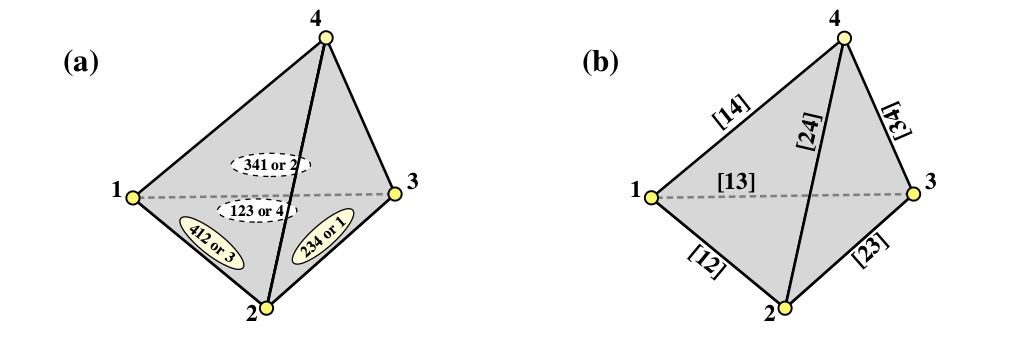
\includegraphics[scale=0.5]{pictures/tetrahedron.png}
\caption[Tetrahedron Conventions]{Naming conventions for tetrahedron faces (a) and edges (b). Courtesy of~\cite{colorado_fem_lectures}}
\end{figure}

\section{Natural Coordinates}

So far we have specified the tetrahedron vertices in Cartesian coordinates $x,y,z$. An alternative coordinate system is called tetrahedral natural coordinates and is composed of four functions: $\Phi^{(1)}(x), \Phi^{(2)}(x), \Phi^{(3)}(x), \Phi^{(4)}(x)$. They value of $\Phi^{(i)}$ is equal to $i$ at vertex $1$ and 0 in all other vertices. We add a constraint:
\begin{equation}
\label{eq:tetra_indentity}
\Phi^{(1)} + \Phi^{(2)} + \Phi^{(3)} + \Phi^{(4)} = 1
\end{equation}

\subsection{Transformation}

We have defined a different coordinate system. However, all quantities such as displacement fields, strain or stress are expressed in Cartesian coordinate system. Thus we need construct a transformation between this two coordinate systems. We combine the identity constraint in Eq~\ref{eq:tetra_indentity} with the linear interpolation of natural coordinates i.e. $x = x_i \Phi^{(i)}$, $y = y_i \Phi^{(i)}$, $z = z_i \Phi^{(i)}$ to get the following matrix relation:

\begin{equation}
\begin{bmatrix}
1 \\
x \\
y \\
z
\end{bmatrix}
=
\begin{bmatrix}
1 & 1 & 1 & 1 \\
x_1 & x_2 & x_3 & x_4 \\
y_1 & y_2 & y_3 & y_4 \\
z_1 & z_2 & z_3 & z_4
\end{bmatrix}
=
\begin{bmatrix}
\Phi^{(1)} \\
\Phi^{(2)} \\
\Phi^{(3)} \\
\Phi^{(4)}
\end{bmatrix}
\end{equation}

The inversion of the above system yields:
\begin{equation}
\begin{bmatrix}
\Phi^{(1)} \\
\Phi^{(2)} \\
\Phi^{(3)} \\
\Phi^{(4)}
\end{bmatrix}
=
\dfrac{1}{6V}
\begin{bmatrix}
6V_{01} & y_{42}z_{32} - y_{32}z_{42} & x_{32}z_{42} - x_{42}z_{32} & x_{42}y_{32} - x_{32}y_{42} \\
6V_{02} & y_{31}z_{43} - y_{34}z_{13} & x_{43}z_{31} - x_{13}z_{34} & x_{31}y_{43} - x_{34}y_{13} \\
6V_{03} & y_{24}z_{14} - y_{14}z_{24} & x_{14}z_{24} - x_{24}z_{14} & x_{24}y_{14} - x_{14}y_{24} \\
6V_{04} & y_{13}z_{21} - y_{12}z_{31} & x_{21}z_{13} - x_{31}z_{12} & x_{13}y_{21} - x_{12}y_{31}
\end{bmatrix}
\begin{bmatrix}
1 \\
x \\
y \\
z
\end{bmatrix}
\end{equation}

The first column is abbreviation for:

\begin{equation}
\begin{aligned}
6V_{01} = x_2(y_3z_4 - y_4z_3) + x_3(y_4z_2 - y_2z_4) +x_4(y_2z_3 - y_3z_2)
\\
6V_{02} = x_1(y_4z_3 - y_3z_4) + x_3(y_1z_4 - y_4z_1) +x_4(y_3z_1 - y_1z_3)
\\
6V_{03} = x_1(y_2z_4 - y_4z_2) + x_2(y_4z_1 - y_1z_4) +x_4(y_1z_2 - y_2z_1)
\\
6V_{04} = x_1(y_3z_2 - y_2z_3) + x_2(y_1z_3 - y_3z_1) +x_3(y_2z_1 - y_1z_2)
\end{aligned}
\end{equation}

It can be shown that $V = V_{01} + V_{02} + V_{03} + V_{04}$.

We can now write the matrix system in more compact way using further abbreviation for the other part of the $4 \times 4$ matrix:

\begin{equation}
\begin{bmatrix}
\Phi^{(1)} \\
\Phi^{(2)} \\
\Phi^{(3)} \\
\Phi^{(4)}
\end{bmatrix}
=
\dfrac{1}{6V}
\begin{bmatrix}
6V_{01} & a_1 & b_1 & c_1 \\
6V_{02} & a_2 & b_2 & c_2 \\
6V_{03} & a_3 & b_3 & c_3 \\
6V_{04} & a_4 & b_4 & c_4
\end{bmatrix}
\begin{bmatrix}
1 \\
x \\
y \\
z
\end{bmatrix}
\end{equation}

The explicit equation for $\Phi^{(i)}$ is given by:
\begin{equation}
\Phi^{(i)} = \dfrac{6V_{0i} + a_i x + b_i y + c_i z}{6V}
\end{equation}

\section{Derivatives}

We can easily compute the following partial derivatives
\begin{equation}
\label{eq:tetra_partial_derivates}
\begin{aligned}
6V \dfrac{\partial \Phi^{(i)}}{\partial x} = 6V \Phi^{(i)}_{,1} = a_i
\\
6V \dfrac{\partial \Phi^{(i)}}{\partial y} = 6V \Phi^{(i)}_{,2} = b_i
\\
6V \dfrac{\partial \Phi^{(i)}}{\partial z} = 6V \Phi^{(i)}_{,3} = c_i
\end{aligned}
\end{equation}

\section{Analytical Integration}

As mentioned before, integration over the linear tetrahedron can be done analytically using the general formula:

\begin{equation}
\int_{\Omega_{e}} \Phi^{i(1)} \Phi^{j(2)} \Phi^{k(3)} \Phi^{l(4)} d \Omega_{e} = \dfrac{i!j!k!l!}{(i+j+k+l+3)!} 6V
\end{equation}

Here the indices without brackets $i,j,k,l$ represent the power exponent.
Special cases that will be of interest for us:
\begin{equation}
\label{eq:anal_intergral}
\begin{aligned}
\int_{\Omega_{e}} d \Omega_{e} = V
\\
\int_{\Omega_{e}} \Phi^{(i)} d \Omega_{e} = \dfrac{1}{4}V
\\
\int_{\Omega_{e}} \Phi^{(i)} \Phi^{(j)} d \Omega_{e} = 
\begin{cases}
\dfrac{1}{10} V \quad i = j 
\\
\dfrac{1}{20} V \quad i \neq j
\end{cases}
\end{aligned}
\end{equation}

We now have all components needed to compute local stiffness matrix $k_{12 \times 12}$ and local force vector $p_{12 \times 1}$. Our natural coordinates $\Phi^{(i)}$ will play a role of shape functions.

\section{Stiffness Matrix}

First, we will define geometric matrix $B$ mentioned in Eq.~\ref{eq:geometric_matrix} explicitely in terms of derivatives computed in Eq.~\ref{eq:tetra_partial_derivates}:

\begin{equation}
\label{eq:geometric_matrix}
B_{6 \times 12} = \dfrac{1}{6V}
\begin{bmatrix}
a_1 & 0 & 0 & a_2 & 0 & 0 & a_3 & 0 & 0 & a_4 & 0 & 0 \\
0 & b_1 & 0 & 0 & b_2 & 0 & 0 & b_3 & 0 & 0 & b_4 & 0 \\
0 & 0 & c_1 & 0 & 0 & c_2 & 0 & 0 & c_3 & 0 & 0 & c_4 \\
b_1 & a_1 & 0 & b_2 & a_2 & 0 & b_3 & a_3 & 0 & b_4 & a_4 & 0 \\
0 & c_1 & b_1 & 0 & c_2 & b_2 & 0 & c_3 & b_3 & 0 & c_4 & b_4 \\
c_1 & 0 & a_1 & c_2 & 0 & a_2 & c_3 & 0 & a_3 & c_4 & 0 & a_4
\end{bmatrix}
\end{equation}

We are going to use the Eq.~\ref{eq:static_fem} with integrals over $\Omega_{e}$. 

First let us compute $k^{(e)}$
\begin{equation}
k^{(e)}_{12 \times 12} = \int_{\Omega_{e}} B^{T}_{6 \times 12} C_{6 \times 6} B_{6 \times 12} dV 
\end{equation}
Since both $B$ and $C$ are constant i.e. do not depend on $x$ we simply get:
\begin{equation}
k^{(e)} = V B^{T} C B 
\end{equation}

\section{Force Vector}
We split the force into two independent parts: body forces and traction forces.

\begin{equation}
\begin{aligned}
p_{12 \times 1} = \int_{\Omega_{e}} \Phi_{3 \times 12}^{T} \hat{f}_{3 \times 1} dV + \int_{\partial \Omega_{\sigma_{e}}} \Phi_{3 \times 12}^{T} \hat{t}_{3 \times 1} dA
\end{aligned}
\end{equation}

\subsection{Body Forces}
Body forces such as gravity, are defined are a single force vector $\hat{f} = \rho[f_1, f_2, f_3]$. This force is applied to all vertices of body and is weighted by the volume of the tetrahedron that the vertex belongs to.
The body force is computed using the fist integral:
\begin{equation}
\begin{aligned}
f^{(e)}_{12 \times 1} = \int_{\Omega_{e}} \Phi_{3 \times 12}^{T} \hat{f}_{3 \times 1} dV
\end{aligned}
\end{equation}
Even if we assume that the body force $\hat{f}$ is constant, $\Phi$ is not constant. It depends on the shape functions $\Phi^{(i)}$ which in turn depends on $x$. Let us define $\Phi$ explicitly:
\begin{equation}
\label{eq:geometric_matrix}
\Phi_{3 \times 12} =
\begin{bmatrix}
\Phi^{(1)} & 0 & 0 & \Phi^{(2)} & 0 & 0 & \Phi^{(3)} & 0 & 0 & \Phi^{(4)} & 0 & 0 \\
0 & \Phi^{(1)} & 0 & 0 & \Phi^{(2)} & 0 & 0 & \Phi^{(3)} & 0 & 0 & \Phi^{(4)} & 0 \\
0 & 0 & \Phi^{(1)} & 0 & 0 & \Phi^{(2)} & 0 & 0 & \Phi^{(3)} & 0 & 0 & \Phi^{(4)} 
\end{bmatrix}
\end{equation}

We can use the second analytical integral presented in Eq.~\ref{eq:anal_intergral}. Assuming that the force $\hat{f} = \rho[f_1, f_2, f_3]$ is constant we receive:
\begin{equation}
\begin{aligned}
f^{(e)}_{12 \times 1} = \dfrac{1}{4} \rho V [f_1, f_2, f_3, f_1, f_2, f_3, f_1, f_2, f_3,f_1, f_2, f_3]^{T} 
\end{aligned}
\end{equation}

\subsection{Traction Forces}
Traction forces simulate the effect of pressure load, e.g. load applied after collision. As opposed to body forces, the traction forces are applied to element faces along their unit normal vector. Thus, each tetrahedron element should have an input of four scalar traction force magnitudes $p_i$, $i=1,2,3,4$, for each face. Traction force for entire tetrahedron is result of a sum of four traction forces computed for each face. To compute traction force for face $1$ or $234$ with input magnitude $p$, we use the formula:
\begin{equation}
\begin{aligned}
t^{(e)}_{12 \times 1} = \dfrac{1}{3} p A_1 [0, 0, 0, \bar{a_1}, \bar{b_1}, \bar{c_1}, \bar{a_1}, \bar{b_1}, \bar{c_1},\bar{a_1}, \bar{b_1}, \bar{c_1}]^{T} 
\end{aligned}
\end{equation}

First we see that the vertex $1$, opposite of face $234$, has received total force equal to $[0,0,0]$. Then, all the other vertices receive the load equally spread among them $\dfrac{1}{3}p A_1$, where $A_1$ is the area of face $234$. Further, the entire vector is directed along the direction cosines $\bar{a_1} = \dfrac{a_1}{S_1}, \bar{b_1} = \dfrac{b_1}{S_1}, \bar{c_1} = \dfrac{c_1}{S_1}$, where $S_1 = \sqrt{a^{2}_{1} + b^{2}_{1} + c^{2}_{1}}$. To compute the area $A_1$ we can use the cross product property. We choose two directed vectors from face $234$ coming from any of its corners e.g. $u_{32} = [x_{32}, y_{32}, z_{32}]$ and $u_{42} = [x_{42}, y_{42}, z_{42}]$. Then:
\begin{equation}
\begin{aligned}
A_1 = \dfrac{1}{2} ||u_{32} \times u_{42}||_{2}
\end{aligned}
\end{equation}

The process is generalized for all face indices $i = 1,2,3,4$.

\section{Mass Matrix}
Recalling the equation~\ref{eq:mass_matrix_matrix} for mass matrix $M$, we can compute the local mass matrix $m^{(e)}$ following the same steps as in the case of stiffness matrix.
\begin{equation}
m^{(e)}_{12 \times 12} =  \int_{\Omega_{e}} \rho \Phi^{T}_{3 \times 12} \Phi_{3 \times 12} dV
\end{equation}

Using the equation~\ref{eq:anal_intergral} we receive:
\begin{equation}
m^{(e)}_{12 \times 12} = \dfrac{\rho V}{20}
\begin{bmatrix}
2 & 0 & 0 & 1 & 0 & 0 & 1 & 0 & 0 & 1 & 0 & 0 \\
0 & 2 & 0 & 0 & 1 & 0 & 0 & 1 & 0 & 0 & 1 & 0 \\
0 & 0 & 2 & 0 & 0 & 1 & 0 & 0 & 1 & 0 & 0 & 1 \\
1 & 0 & 0 & 2 & 0 & 0 & 1 & 0 & 0 & 1 & 0 & 0 \\
0 & 1 & 0 & 0 & 2 & 0 & 0 & 1 & 0 & 0 & 1 & 0 \\
0 & 0 & 1 & 0 & 0 & 2 & 0 & 0 & 1 & 0 & 0 & 1 \\
1 & 0 & 0 & 1 & 0 & 0 & 2 & 0 & 0 & 1 & 0 & 0 \\
0 & 1 & 0 & 0 & 1 & 0 & 0 & 2 & 0 & 0 & 1 & 0 \\
0 & 0 & 1 & 0 & 0 & 1 & 0 & 0 & 2 & 0 & 0 & 1 \\
1 & 0 & 0 & 1 & 0 & 0 & 1 & 0 & 0 & 2 & 0 & 0 \\
0 & 1 & 0 & 0 & 1 & 0 & 0 & 1 & 0 & 0 & 2 & 0 \\
0 & 0 & 1 & 0 & 0 & 1 & 0 & 0 & 1 & 0 & 0 & 2 \\
\end{bmatrix}
\end{equation}

Similarly to stiffness, mass matrix is also symmetric.

\subsection{Mass Matrix Diagonalization}
TODO

% ---------------------------------------------------
\chapter{Solving System of Linear Equations}
\label{chap:system_linear}

\section{Conjugate Gradient}
This section explains all the tools required to define the Conjugate Gradient algorithm.
\subsection{Introduction}
Conjugate Gradient(CG) is one of the most popular iterative methods of solving system of linear equations:
\begin{equation}
Ax=b
\end{equation}
where $A$ is a square $n \times n$, symmetric, positive-definite(or positive-indefinite) matrix, $x$ and $b$ are vectors e.i. $n \times 1$ matrices
We define inner product(also known as dot product) of vector by 
\begin{equation}
x^{T}y = \sum^{n}_{i=1} x_i y_i
\end{equation}

Two vector $x$ and $y$ are said to be orthogonal when:
\begin{equation}
x^{T}y = 0
\end{equation}

A matrix $A$ is positive-definite if for every nonzero vector x:
\begin{equation}
x^{T}Ax > 0
\end{equation}

\subsection{Quadratic Form}
A quadratic form a scalar function of a vector:
\begin{equation}
\label{eq:quadratic_form}
f(x) = \dfrac{1}{2}x^{T}Ax - b^{T}x + c
\end{equation}
where $A$ is matrix, $x$ and $b$ are vector and c is a scalar.
Gradient of quadratic form is defined:
\begin{equation}
\label{eq:gradient_f}
f^{'}(x) = 
\begin{bmatrix}
\dfrac{\partial}{\partial x_1} f(x) \\
\dfrac{\partial}{\partial x_2} f(x) \\
. \\
. \\
. \\
\dfrac{\partial}{\partial x_n} f(x)
\end{bmatrix}
\end{equation}

Taking a gradient of Eq.~\ref{eq:quadratic_form} yields:
\begin{equation}
f^{'}(x) = \dfrac{1}{2}A^{T}x + \dfrac{1}{2}Ax - b
\end{equation}
If $A$ is symmetric then:
\begin{equation}
f^{'}(x) = Ax - b
\end{equation}
If we set the gradient to zero then we get the solution for $Ax=b$ which is also a critical point of $f(x)$. If $A$ is also positive-definite then this solution is also a minimum of $f(x)$. In other words, to solve $Ax=b$, we can find such an $x$ that minimizes $f(x)$.

\begin{figure}[h!]
\centering
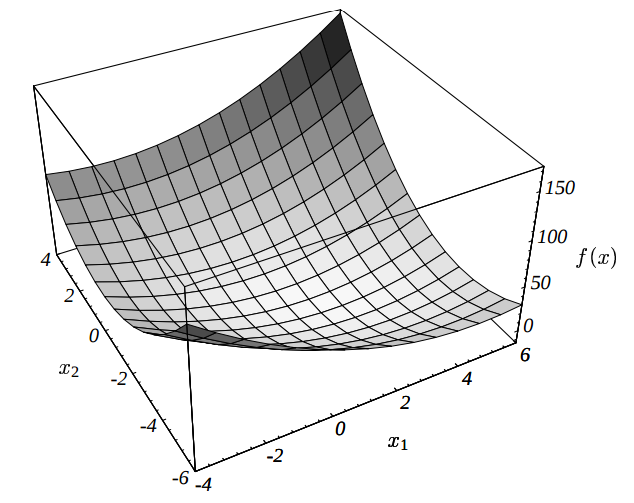
\includegraphics[scale=0.5]{pictures/paraboloid.png}
\caption[Paraboloid of quadratic form]{Paraboloid of example quadratic form f(x). Courtesy of~\cite{cg}}
\end{figure}

\begin{figure}[h!]
\centering
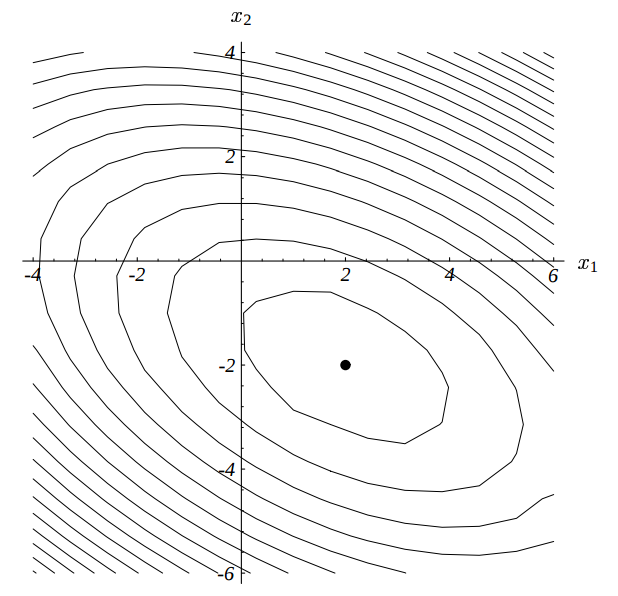
\includegraphics[scale=0.5]{pictures/contour.png}
\caption[Contour plot of quadratic form]{Contour plot of example quadratic form f(x). Courtesy of~\cite{cg}}
\end{figure}

\subsection{Steepest Descent}
In the method of Steepest Descent we look for the solution $x$ by going down the paraboloid. We start at some point $x_0$ and iterate the steps taking new points $x_1, x_2 ,...$ until we hit the minimum. Obviously we want to take the steps in the direction for which values of $f$ decreases the most. That direction is the opposite of $f^{'}(x)$, namely:
\begin{equation}
\label{eq:gradient_minus}
-f^{'}(x) = b - Ax
\end{equation}

Let us define a few measurements. The error:
\begin{equation}
e_i = x_i - x
\end{equation}
Error vector $e_i$ shows the distance, in a given iteration $i$, from the solution $x$.

The residual:
\begin{equation}
\label{eq:residual}
r_i = b - Ax_i
\end{equation}
Residual vector $r_i$ shows the distance, in a given iteration $i$, from correct value $b$.
Combining equations~\ref{eq:residual} and~\ref{eq:gradient_minus} we get:
\begin{equation}
r_i = -f^{'}(x_i)
\end{equation}
That means that the residual is the direction of steepest descent. Thus the next step $x_i$ is defined as:
\begin{equation}
x_{i+1} = x_{i} + \alpha r_{i}
\end{equation}
New issue arises, namely computing the length of direction vector $r_{i}$: $\alpha$.
We use a line search that will choose $\alpha$ that minimizes $f$ along a line. Figures~\ref{fig:cg_alpha1} and~\ref{fig:cg_alpha1} show an example case of finding alpha. First in figure~\ref{fig:cg_alpha1} we see the intersection of a paraboloid and a surface defined by some initial point $x_0$ and the direction of steepest descent. Figure~\ref{fig:cg_alpha2} shows the parabola of this intersection, which helps us to see what is the value of $\alpha$ at the base of the parabola. This is obviously the case when the derivative $\dfrac{d}{d\alpha}f(x_{i+1})$ is equal to zero. We can use the chain rule to further compute:
\begin{equation}
\dfrac{d}{d \alpha}f(x_{i+1}) = f^{'}(x_{i+1})^{T} \dfrac{d}{d \alpha} x_{i+1} = f^{'}(x_{i+1})^{T} r_i
\end{equation}

Setting the expression $f^{'}(x_{1i+1})^{T} r_i$ to zero means that $f^{'}(x_{i+1})^{T}$ and  $r_i$ have to orthogonal.
Formally, computing $\alpha$ goes as follows:
\begin{equation}
\begin{aligned}
r^{T}_{i+1}r_{i} = 0
\\
(b - Ax_{i+1})^{T}r_{i} = 0
\\
(b - A(x_{i} + \alpha r_{i}))^{T}r_{i} = 0
\\
(b - Ax_{i})^{T}r_{i} - \alpha (Ar_{i})^{T}r_{i}= 0
\\
(b - Ax_{i})^{T}r_{i} = \alpha (Ar_{i})^{T}r_{i}
\\
r_{i}^{T}r_{i} = \alpha r_{i}^{T} (Ar_{i})
\\
\alpha = \dfrac{r_{i}^{T}r_{i}}{r_{i}^{T} (Ar_{i})}
\end{aligned}
\end{equation}

\begin{figure}[h!]
\centering
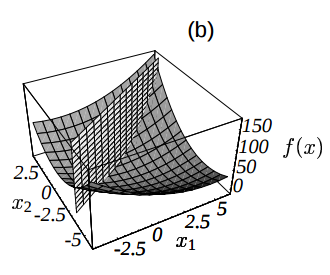
\includegraphics[scale=0.8]{pictures/alpha1.png}
\caption[Paraboloid and surface]{Paraboloid and a surface defined by residual direction at some step. Courtesy of~\cite{cg}}
\label{fig:cg_alpha1}
\end{figure}

\begin{figure}[h!]
\centering
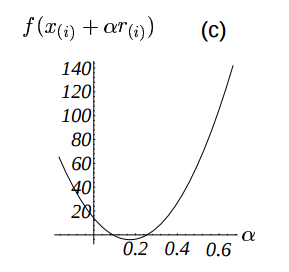
\includegraphics[scale=0.8]{pictures/alpha2.png}
\caption[Intersection of paraboloid and surface]{The intersection parabola of two surfaces shown in~\ref{fig:cg_alpha1}. Courtesy of~\cite{cg}}
\label{fig:cg_alpha2}
\end{figure}

The entire Steepest Descent algorithm can be summarized as follows:

\begin{equation}
\begin{aligned}
r_{i} = b - Ax_{i}
\\
\alpha_{i} = \dfrac{r_{i}^{T}r_{i}}{r_{i}^{T} (Ar_{i})}
\\
x_{i+1} = x_{i} + \alpha_{i}r_{i}
\end{aligned}
\end{equation}

Example solution of Steepest Descent is shown in figure~\ref{fig:steepest_descent}

\begin{figure}[h!]
\centering
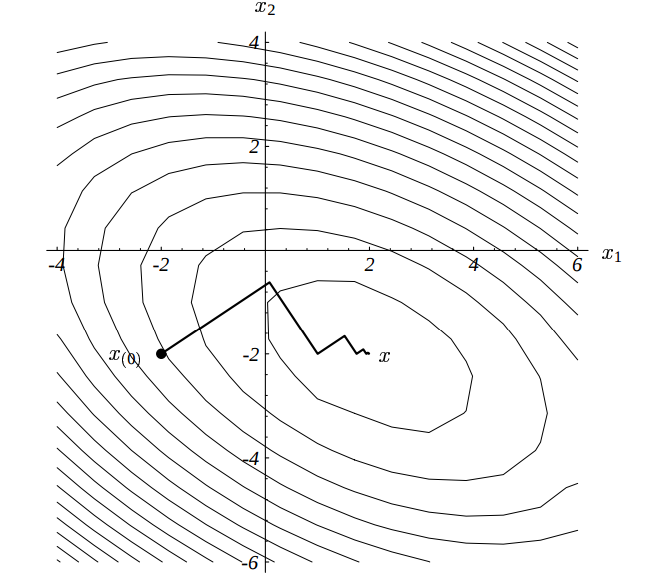
\includegraphics[scale=0.5]{pictures/steepest_descent.png}
\caption[Steepest Descent steps]{Example of Steepest Descent solution. Courtesy of~\cite{cg}}
\label{fig:steepest_descent}
\end{figure}

\subsection{Conjugate Directions}
Iterations in Steepest Descent method usually end up taking the same directions as one of the previous iterations, see figure~\ref{fig:steepest_descent}. Conjugate Direction method chooses a set of orthogonal search directions $d_0, d_1,...,d_{n-1}$. Taking next step looks now as follows:
\begin{equation}
\begin{aligned}
x_{i+1} = x_{i} + \alpha_{i}d_{i}
\end{aligned}
\end{equation}

Generating the set of directions $\{ d_i \}$ is done using the process called conjugate Gram-Schmidt. Assume we have $n$ linearly independent vectors $u_0, u_1, ..., u_{n-1}$. We construct $d_i$ using the formula:
\begin{equation}
d_{i} = u_{i} + \sum^{i-1}_{k=0} \beta_{ik} d_{k}
\end{equation}
where $\beta_{ij}$ is defined by:
\begin{equation}
\beta_{ij} = - \dfrac{u^{T}_i A d_{j}}{d^{T}_{j}A d_{j}}
\end{equation}

\subsection{Conjugate Gradient}
Finally we can define the Conjugate Gradient method. CG is a special case of Conjugate Directions method using $u_i = r_i$. The equations required to compute CG are presented:

\begin{equation}
\begin{aligned}
d_0 = r_0 = b - Ax_0
\\
\alpha_i = \dfrac{r^{T}_{i} r_{i}}{d^{T}{i} A d_{i}}
\\
x_{i+1} = x_{i} + \alpha_{i}d_{i}
\\
r_{i+1} = r_{i} - \alpha_{i}Ad_{i}
\\
\beta_{i+1,i} = - \dfrac{r^{T}_{i+1} r_{i+1}}{r^{T}_{i} r_{i}}
\\
d_{i+1} = r_{i+1} + \beta_{i+1,i} d_{i}
\end{aligned}
\end{equation}
The most expensive operation in CG is the matrix-vector multiplication which in general has time complexity of $\mathcal{O}(m)$, where $m$ is the number of non-zero elements in $A$. This means that each iterations of CG method has time complexity $\mathcal{O}(m)$.

The algorithm ends when maximum number of iteration has been reached or when $r_i$ is small enough.

% ---------------------------------------------------
\chapter{Tetrahedralization}
\label{chap:Tetrahedralization}

A quality mesh can be defined by a few properties.
One of the most basic properties is the fact that generated 3D mesh should correctly model the shape of the input domain. Figure~\ref{fig:mesh_incomplete} shows an tetrahedron mesh that does not model the shape of the cube domain correctly.

\begin{figure}[h!]
\centering
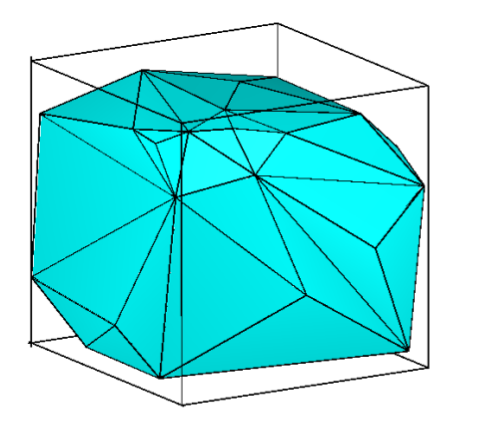
\includegraphics[scale=0.5]{pictures/3dmesh_incomplite.png}
\caption[Poor 3D mesh]{Example 3D tetrahedron mesh that does not correctly model the domain of the cube. Courtesy of~\cite{delaunay_mesh}}
\label{fig:mesh_incomplete}
\end{figure}

Second important property is the control of individual elements size. Controlling the volume of elements enables the user to control the accuracy of computations. Bigger number of smaller elements can lead to more accurate but slower computations.

Another problem that has to be solved is the control of elements shape. We often want our tetrahedra to have regular shapes. Meaning that extreme angle values should be avoided. We can ensure the regular shape by controlling the lower bound of the smallest angle in a tetrahedron which also controls the largest angle. Some examples of tetrahedron shapes are shown in figure~\ref{fig:tetrahedra_shapes}.

\begin{figure}[h!]
\centering
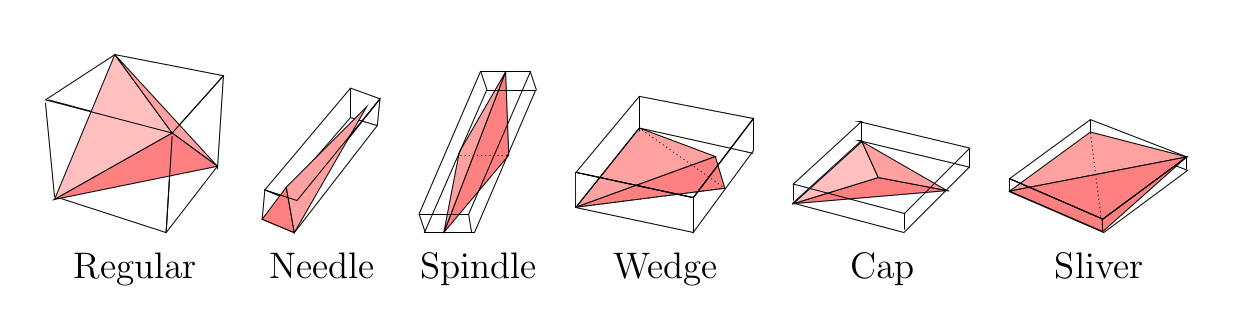
\includegraphics[scale=0.3]{pictures/tetrahedra_shapes.png}
\caption[Tetrahedron shapes]{Example of some common tetrahedron shapes. Courtesy of~\cite{tetgen}}
\label{fig:tetrahedra_shapes}
\end{figure}

\begin{figure}[h!]
\centering
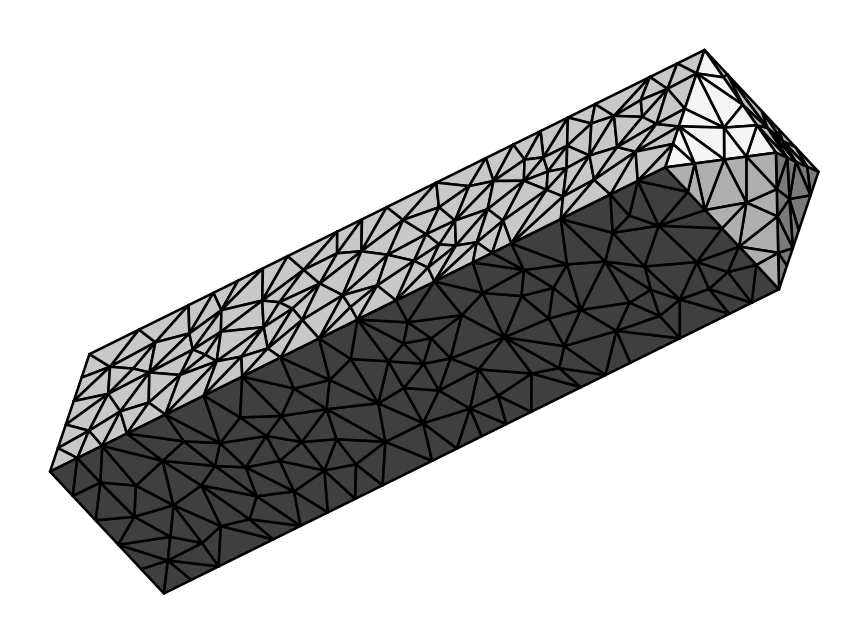
\includegraphics[scale=0.5]{pictures/3dmesh.png}
\caption[Fine tetrahedron mesh]{Example 3D tetrahedron mesh. Courtesy of~\cite{delaunay_mesh}}
\end{figure}

\section{Piecewise Linear Complexes}
\label{sec:plc}

\section{The Delaunay Triangulation}

\section{Two-Dimensional Delaunay Refinement}

\section{Three-Dimensional Delaunay Refinement}

%-----------------------------------------------------------------
\chapter{Implementation}
\label{chap:Implementation}

The implementation of this thesis has two parts: numerical library and 3D graphic engine. The numerical library contains all the tools to compute real time finite element method solver. The library is then integrated into a demo 3D engine.

\section{RTFEM}
RTFEM stands for Real-Time Finite Element Method. The library computes the entire process of FEM for solid mechanics:
\begin{enumerate}
\item Pre-Processing: 3D Finite Element Meshing
\item Solver: CPU and GPU dynamic, linear FEM Solver.
\item Post-Processing: Output the displacements.
\end{enumerate}

RTFEM was written in c++11 and uses general template programming. Template programming is used to allow the user to easily change the precision between float and double. RTFEM can be built on any platform supporting cmake. All the tests were made on 64bit Arch Linux. The source code is available in~\cite{rtfem}.

\subsection{Folder Structure}
RTFEM folder structure looks as follows:
\begin{enumerate}
\item /documentation - library documentation
\item /external - all the external libraries
\item /sources - sources code of the library
\item /tests - unittests
\end{enumerate}
For more information about building the library see ReadMe.md in root directory.

\subsection{External Libraries}
RTFEM uses the following external libraries:
\begin{enumerate}
\item TeTGen~\cite{tetgen}: 3D Tetrahedron meshing algorithm.
\item Eigen~\cite{eigen}: CPU Matrix operations and System of Linear Equation Solver
\item CUBLAS~\cite{cublas}, CUSPARSE~\cite{cusparse}: GPU Matrix operations and System of Linear Equation Solver
\item googletest~\cite{googletest}: Unit test framework.
\end{enumerate}

\subsection{Architecture}
Let us start by describing the architecture of the library. First, the data structures used to represented the FEM model are shown in figure~\ref{fig:uml_fem_model}. FEMModel class is the main container of all sub-components. It also enabled the user to set up body force which acts on all vertices in the model. FEMGeometry holds all the information about geometry of 3D tetrahedron mesh. Vertex is defined by and id and coordinates. TriangleFace is defined by three pointers to vertices. Moreover it contains information about its area, whether it is boundary face and current traction force applied to it. User can apply traction forces directly to the triangle faces. FiniteElement contains pointers to vertices and faces. It also stores information about its volume. Material class is used to store the information of physical material used in the simulation. The variables $damping\_mass$ and $damping\_stiffness$ are used to compute damping matrix $C$ and correspond to $\alpha$ and $\beta$ from Eq.~\ref{eq:damping_matrix}. Finally the BoundaryCondition is used to store information about a single boundary condition. User defines the vertex id and the value which this vertex should take.

\begin{figure}[h!]
\centering
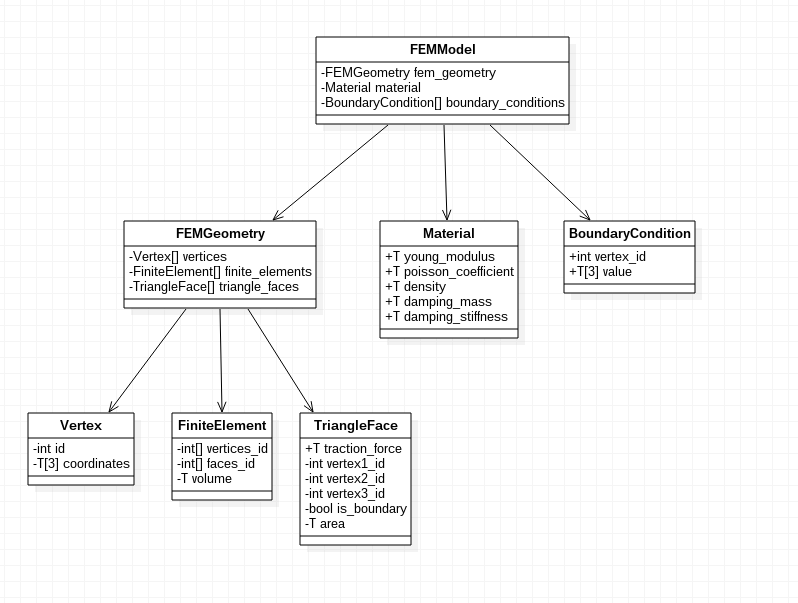
\includegraphics[scale=0.6]{pictures/fem_model.png}
\caption[Class diagram of RTFEM data structures]{Class diagram of RTFEM data structures}
\label{fig:uml_fem_model}
\end{figure}

The post processing part, namely the 3D mesh generation, is mostly done by TeTGen library. The figure~\ref{fig:uml_tetrahedralization} shows the simply process. TriangleMesh is composed by a set of vertices and faces. Such a triangle mesh can be easily converted from any triangle mesh used in 3D graphics libraries such as OpenGL. Moreover, this triangle mesh is assumed to be a closed mesh. Such a triangle mesh can be easily described as PLC explained in section~\ref{sec:plc}. The Tetrahedralization class computes and outputs FEMGeometry.

\begin{figure}[h!]
\centering
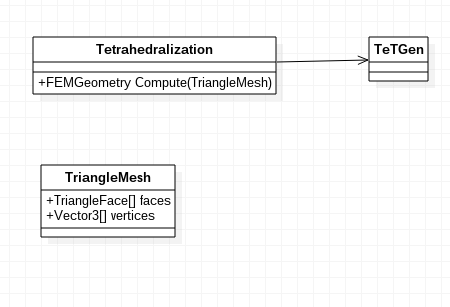
\includegraphics[scale=0.6]{pictures/tetrahedralization.png}
\caption[Class diagram of RTFEM tetrahedralization process]{Class diagram of RTFEM tetrahedralization process}
\label{fig:uml_tetrahedralization}
\end{figure}

The solver part of the system is presented in figure~\ref{fig:uml_solver}. First, the FEMGlobalDynamicAssembler and TetrahedronLocalAssembler are used to assemble all the required components and store them in FEMGlobalAssemblerData. GPUMVSparseMultiplication is used for the sparse matrix-vector multiplication. GPUSparseCGLinearSolver is the sparse conjugate gradient solver. FEMDynamicSolver class is in the center of the entire solver system. It pre-computes and stores all required data and runs computations for each iteration. The solver uses implicit euler integration method as described in section~\ref{sec:ImplicitEuler}. The output displacements are stored in FEMSolverOutput class.

\begin{figure}[h!]
\centering
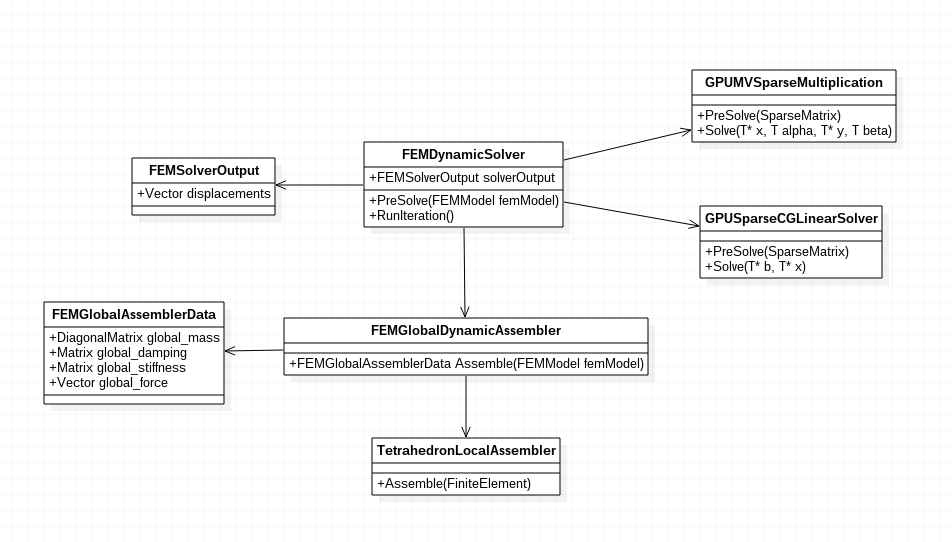
\includegraphics[scale=0.5]{pictures/solver.png}
\caption[Class diagram of solver]{Class diagram of solver}
\label{fig:uml_solver}
\end{figure}

\subsection{Solver Algorithms}
The FEMDynamicSolver has to public functions: PreSolve and RunIteration. PreSolve is used to compute and store all the constant data that are used throughout all iterations. Algorithm~\ref{alg:presolver} shows the necessary steps.

\begin{algorithm}
\caption{FEM Dynamic Solver: PreSolver}
\label{alg:presolver}
\begin{algorithmic}[1]
\Procedure{PreSolve}{}
\State InitAssembly()
\State InitDisplacementData()
\State InitPreSolveLHS()
\State InitPreSolveRHS()
\EndProcedure
\end{algorithmic}
\end{algorithm}

InitAssembly algorithm~\ref{alg:InitAssembly} computes the assembly process and stores an instance of FEMGlobalAssemblerData.

\begin{algorithm}
\caption{FEM Dynamic Solver: InitAssembly}
\label{alg:InitAssembly}
\begin{algorithmic}[1]
\Procedure{InitAssembly}{}
\State femAssemblerData = FEMGlobalDynamicAssembler.Compute(femModel)
\EndProcedure
\end{algorithmic}
\end{algorithm}

InitDisplacementData simply creates new zero vectors, see algorithm~\ref{alg:InitDisplacementData}.
 
\begin{algorithm}
\caption{FEM Dynamic Solver: InitDisplacementData}
\label{alg:InitDisplacementData}
\begin{algorithmic}[1]
\Procedure{InitDisplacementData}{}
\State displacementVelocityCurrent = new Vector()
\State displacementPositionCurrent = new Vector()
\EndProcedure
\end{algorithmic}
\end{algorithm}

InitPreSolveLHS presented in algorithm~\ref{alg:InitPreSolveLHS} computes left hand side(LHS) of the system shown in section~\ref{sec:ImplicitEuler} and transforms it to sparse CSR format. Then, the boundary conditions are applied but only to matrix LHS, since the force vector will change every iteration. Finally, the sparse matrix LHS is stored on the GPU using the GPUSparseCGLinearSolver class. 

\begin{algorithm}
\caption{FEM Dynamic Solver: InitPreSolveLHS}
\label{alg:InitPreSolveLHS}
\begin{algorithmic}[1]
\Procedure{InitPreSolveLHS}{}
\State LHS = ComputeLHS()
\State TransformToSparse(LHS)
\State ApplyBoundaryConditionsMatrix(LHS, boudaryConditions)
\State GPUSparseCGLinearSolver.PreSolve(LHS)
\EndProcedure
\end{algorithmic}
\end{algorithm}

InitPreSolveRHS in algorithm~\ref{alg:InitPreSolveRHS} pre-computes the right hand side vector. It transforms global mass and global stiffness matrices to sparse CSR formats and stores them on the GPU using GPUMVSparseMultiplication class.

\begin{algorithm}
\caption{FEM Dynamic Solver: InitPreSolveRHS}
\label{alg:InitPreSolveRHS}
\begin{algorithmic}[1]
\Procedure{InitPreSolveRHS}{}
\State TransformToSparse(globalMass)
\State GPUMVSparseMultiplicationMass.PreSolve(globalMass)
\State TransformToSparse(globalStiffness)
\State GPUMVSparseMultiplicationStiffness.PreSolve(globalStiffness)
\EndProcedure
\end{algorithmic}
\end{algorithm}

Computations for each iteration are shown in algorithm~\ref{alg:RunIteration}. ReAssembleForces process, simply gathers the traction and body forces and re assembles them into the force vector. ResetForces, resets them back to zero.

\begin{algorithm}
\caption{FEM Dynamic Solver: RunIteration}
\label{alg:RunIteration}
\begin{algorithmic}[1]
\Procedure{RunIteration}{}
\State ReAssembleForces()
\State SolveForDisplacements()
\State ResetForces()
\EndProcedure
\end{algorithmic}
\end{algorithm}

SolveForDisplacements function shown in algorithm~\ref{alg:SolveForDisplacements} computes the implicit euler integration method. First we compute the right hand side vector using the two GPUMVSparseMultiplication classes initiated in the pre solver. We apply the boundary conditions to the RHS. Then we are ready to run the conjugate gradient solver on the GPU to solve our system for velocities. New velocities are used in integration to compute new displacement vector.

\begin{algorithm}
\caption{FEM Dynamic Solver: SolveForDisplacements}
\label{alg:SolveForDisplacements}
\begin{algorithmic}[1]
\Procedure{SolveForDisplacements}{}
\State RHS = ComputeRHS()
\State ApplyBoundaryConditionsVector(RHS, boundaryConditions);
\State newVelocity = GPUSparseCGLinearSolver.Solve(RHS);
\State Integrate(newVelocity);
\EndProcedure
\end{algorithmic}
\end{algorithm}

Computing right hand side vector and solving linear system of equations require the most computation power. These two functions are fully accelerated on GPU using CUDA.

\section{RTFEM Integration into Game Engine}
For the purposes of this thesis RTFEM has been integrated into open source game engine created by the author of this thesis, see source code~\cite{ifx}. The entire architecture of the engine is out of the scope of this text. However, the following section will describe the components needed to understand the process of integrating RTFEM. Figure~\ref{fig:ifx_example} shows screenshot from the engines editor.

\begin{figure}[h!]
\centering
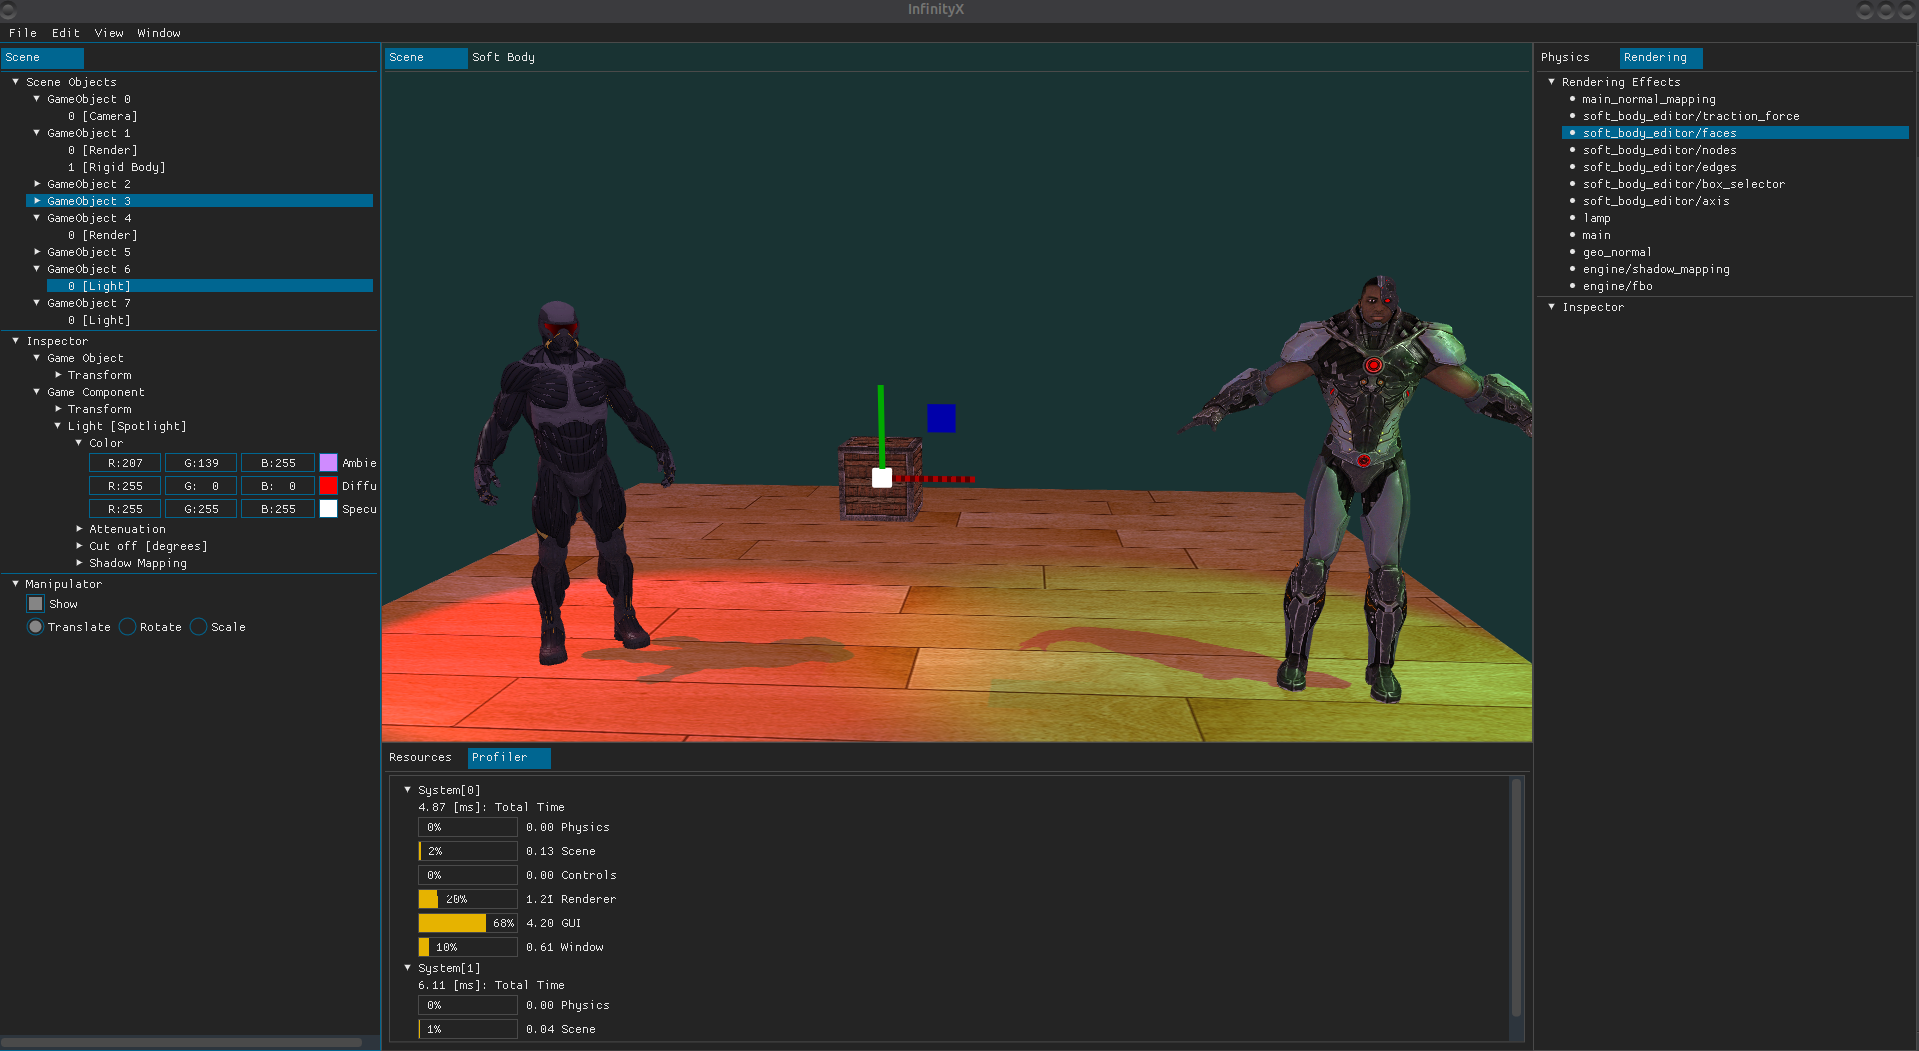
\includegraphics[scale=0.2]{pictures/ifx/ifx.png}
\caption[Game engine]{Game engine~\cite{ifx}}
\label{fig:ifx_example}
\end{figure}

Figure~\ref{fig:ifx_general} shows the most important modules. Physics module is devoted to run rigid body and soft body simulations. For rigid body simulations it encapsulates lower level rigid body libraries such as PhysX 3.4~\cite{physx} and Bullet~\cite{bullet}. Soft body simulation is implemented using RTFEM.
Graphics module is built on top of OpenGL~\cite{opengl}. It encapsulates low level OpenGL programming to increase the productivity. It supports rendering with basic texture materials such as diffuse, ambient and normal mapping. It also supports lighting and shadow effects. User can easily program and edit shader program in run time.
InputControls is a module responsible for handling user input from mouse and keyboard.
Game module combines all individual modules and provides set of rules for how they should interact with each other. All modules are fully decoupled and communicate with each other through Game module.
Finally, Editor module is responsible for graphical user interface, which allows for creating 3D objects, rigid bodies, editing shaders and soft body objects.

\begin{figure}[h!]
\centering
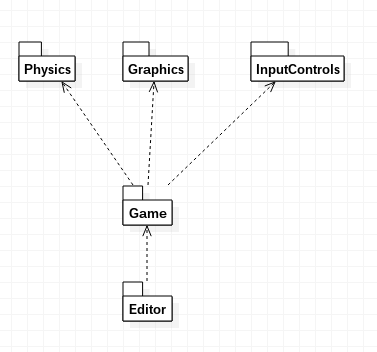
\includegraphics[scale=0.5]{pictures/ifx_general.png}
\caption[Game engine modules overview]{Game engine modules overview}
\label{fig:ifx_general}
\end{figure}

Physics module is described in more detail in figure~\ref{fig:ifx_physics}. RigidBody and RigidBodySimulation use the bridge design pattern to inject different implementations such as PhysX, Bullet or other libraries that the user might want to implement. SoftBodySimulation uses FEMDynamicSolver to simulate physics for SoftBodyFEM objects.

\begin{figure}[h!]
\centering
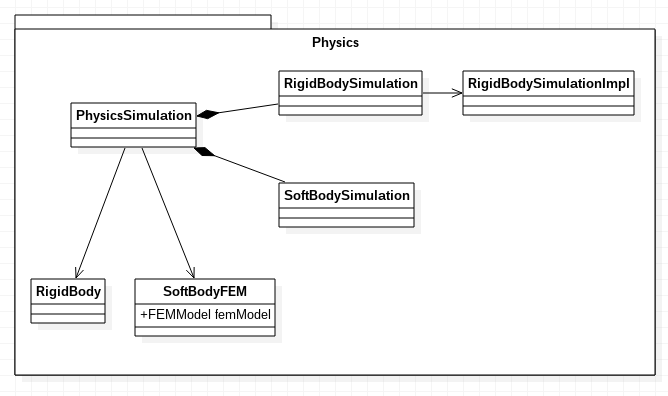
\includegraphics[scale=0.5]{pictures/ifx_physics.png}
\caption[Game engine physics module]{Game engine physics module}
\label{fig:ifx_physics}
\end{figure}

Most important systems of Graphics module is shown in figure~\ref{fig:ifx_graphics}. Renderer contains RenderingEffects which are composed of RenderObjects and ShaderPrograms. RenderObject encapsulates the triangle mesh and materials such textures and other parameters. ShaderProgram interprets these triangles meshes and materials by programmable shaders using GLSL language.

\begin{figure}[h!]
\centering
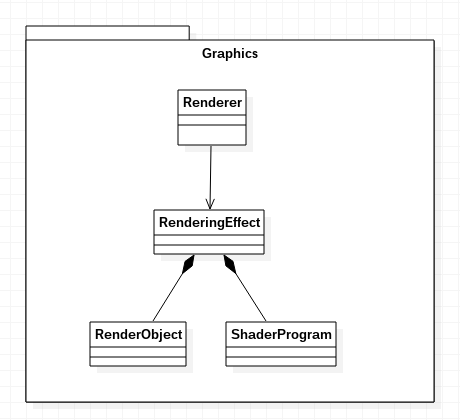
\includegraphics[scale=0.5]{pictures/ifx_graphics.png}
\caption[Game engine graphics module]{Game engine graphics module}
\label{fig:ifx_graphics}
\end{figure}

Basic GameLoop is presented in figure~\ref{fig:ifx_game1}. The GameContainer contains GameObjects which are composed of GameComponents. GameObject are object that appear in the scene. They can be transformed to any coordinate system by translation, rotation or scaling. We add GameComponents to make the game objects more interesting. Currently the engine supports multiple game components: light source, camera, render object, rigid body or soft body.

\begin{figure}[h!]
\centering
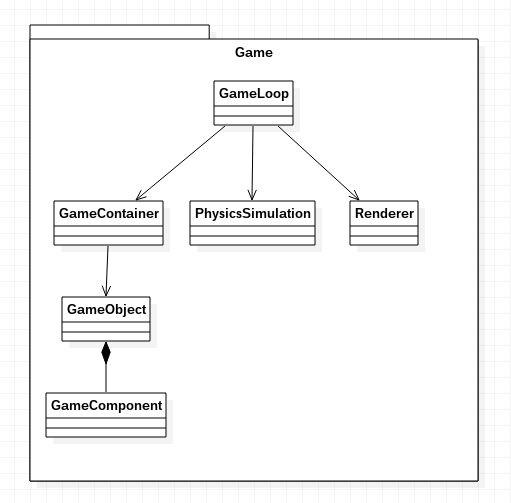
\includegraphics[scale=0.5]{pictures/ifx_game.png}
\caption[Game engine game module]{Game engine game module}
\label{fig:ifx_game1}
\end{figure}

The game loop sequence is shown in figure~\ref{fig:ifx_game_loop}. Each system is updated in a sequence. However each system is updated with different frequency, which can be set by the user. For example, we can update physics twice as often as rendering graphics. GameContainer update is used to synchronize transformations of rigid bodies computed in physics simulation with render components.

\begin{figure}[h!]
\centering
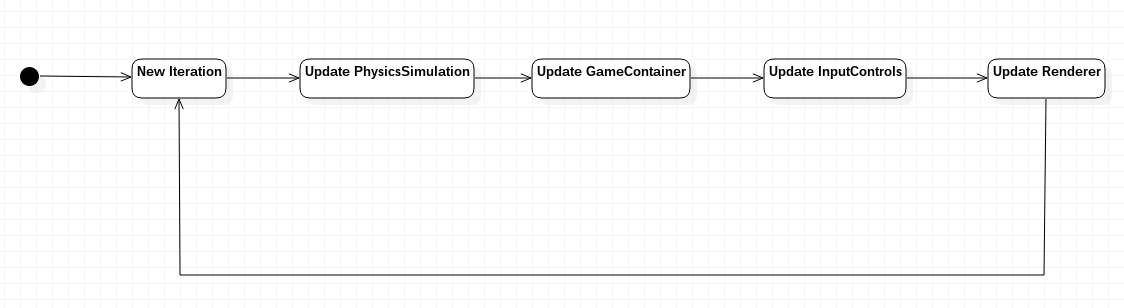
\includegraphics[scale=0.4]{pictures/game_loop.png}
\caption[Game engine game loop sequence]{Game engine game loop sequence}
\label{fig:ifx_game_loop}
\end{figure}

Finally, figure~\ref{fig:ifx_game2} described the integration of soft body into game module. SoftBodyFEMComponent is created by deriving the GameComponent interface and SoftBodyFEM from the physics module. The soft body component also contains a render object which is created by fetching the boundary triangle faces of FEM model. SoftBodyFEM is updated in PhysicsSimulation which computes and stores the displacements. SoftBodyFEMComponent uses the displacements to synchronize render-able vertices by updating the current vertex buffer object(VBO). That happens in the GameContainer update function. Finally the boundary triangle faces are rendered in Renderer update.

\begin{figure}[h!]
\centering
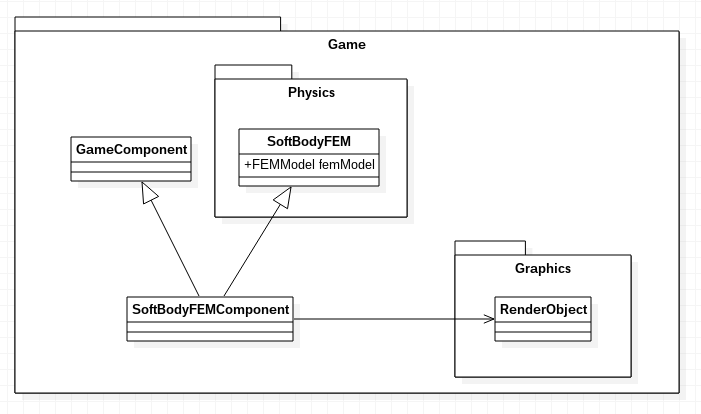
\includegraphics[scale=0.5]{pictures/ifx_game2.png}
\caption[Game engine game module. Soft body integration]{Game engine game module. Soft body integration}
\label{fig:ifx_game2}
\end{figure}


\subsection{Editor}
This section describes the graphical editor of soft body system in the game engine. Soft body editor can be opened by clicking the Soft Body button located in the middle view port, see figure~\ref{fig:ifx_example}. We can select a game object to be opened by right clicking it in the scene list(left panel). Game object that can be opened in the soft body editor must have exactly one render component. It can have other components too. The render component contains the triangle mesh that is used as a input problem domain in the 3D mesh generation. Figures~\ref{fig:ifx_meshing} through~\ref{fig:ifx_solver2} present the soft body editor panels. In the first step we want to create 3D mesh. Meshing panel is devoted to that procedure. Figure~\ref{fig:ifx_meshing} shows control parameters explained in chapter~\ref{chap:Tetrahedralization}. The cube has been already meshes with example parameter values.


\begin{figure}[h!]
\centering
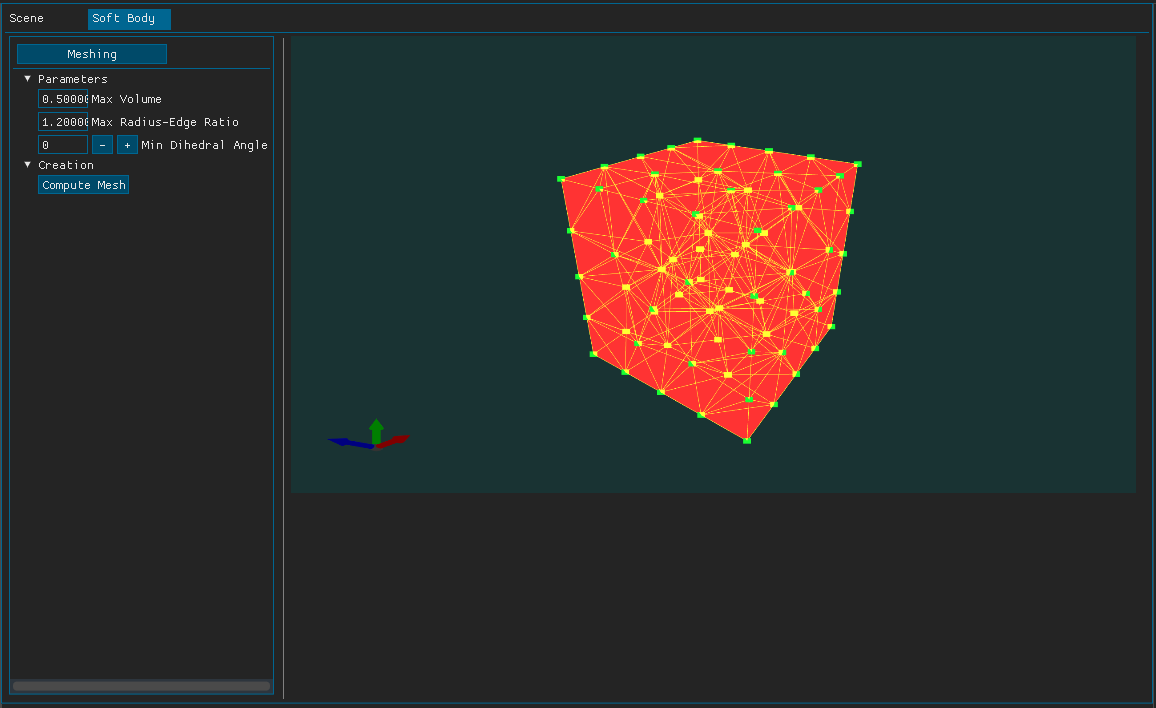
\includegraphics[scale=0.3]{pictures/ifx/ifx_meshing.png}
\caption[Soft body editor. Meshing panel]{Soft body editor. Meshing panel}
\label{fig:ifx_meshing}
\end{figure}

Next, figure~\ref{fig:ifx_material}, we are presented with materials described in chapter~\ref{chap:solid_mechanics1}.

\begin{figure}[h!]
\centering
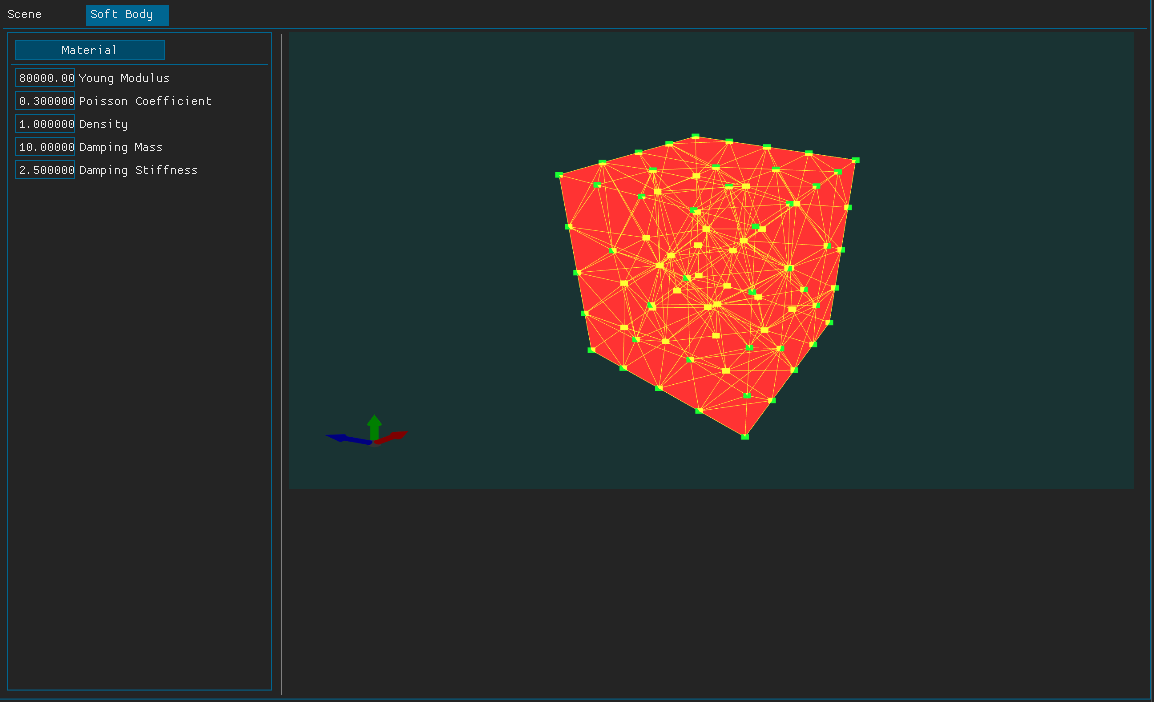
\includegraphics[scale=0.3]{pictures/ifx/ifx_material.png}
\caption[Soft body editor. Material panel]{Soft body editor. Meshing panel}
\label{fig:ifx_material}
\end{figure}

Boundary conditions panel is shown in figure~\ref{fig:ifx_bc}. The user can select multiple vertices by holding down the left mouse button. Then the user inputs the value for new boundary conditions. In this example, the velocity of selected vertices will be equal to zero. Thus, the vertices will stay put.

\begin{figure}[h!]
\centering
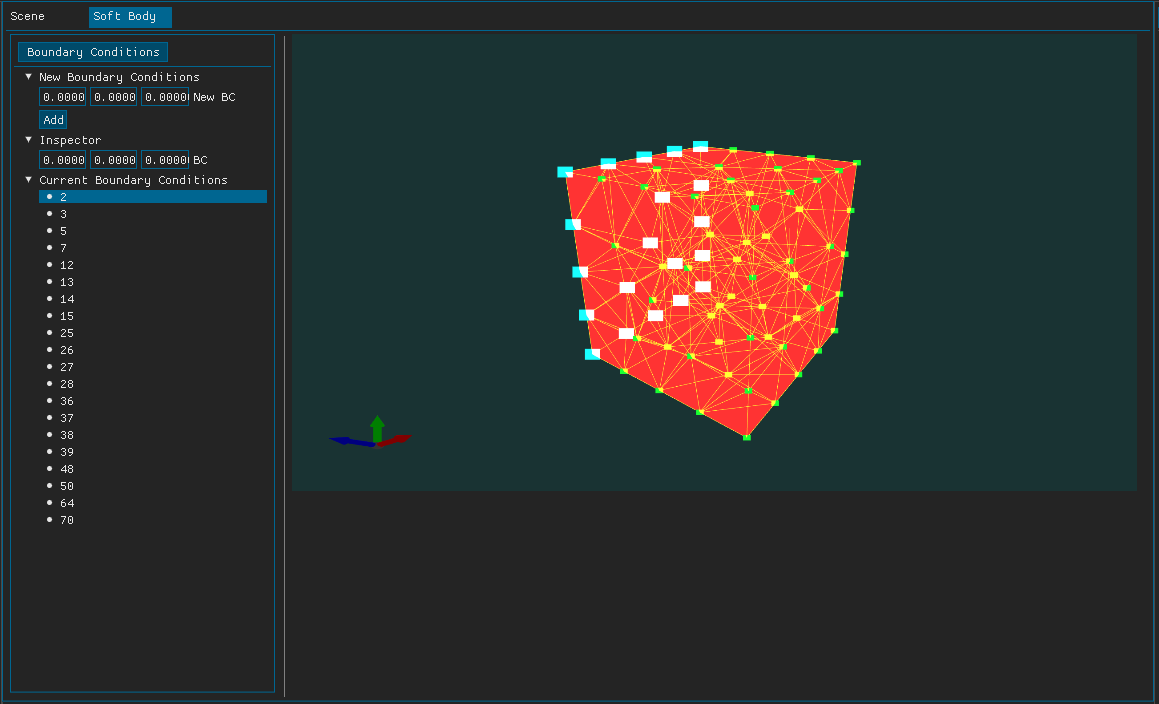
\includegraphics[scale=0.3]{pictures/ifx/ifx_bc.png}
\caption[Soft body editor. Boundary conditions panel]{Soft body editor. Boundary conditions panel}
\label{fig:ifx_bc}
\end{figure}

In the load panel(see figure~\ref{fig:ifx_load} user can select body force that acts on the entire body, simulating gravity. Traction forces are selected by left clicking on a triangle face and dragging the mouse to choose the magnitude of traction force. Remember that the direction of the traction force lies along the normal of that face.

\begin{figure}[h!]
\centering
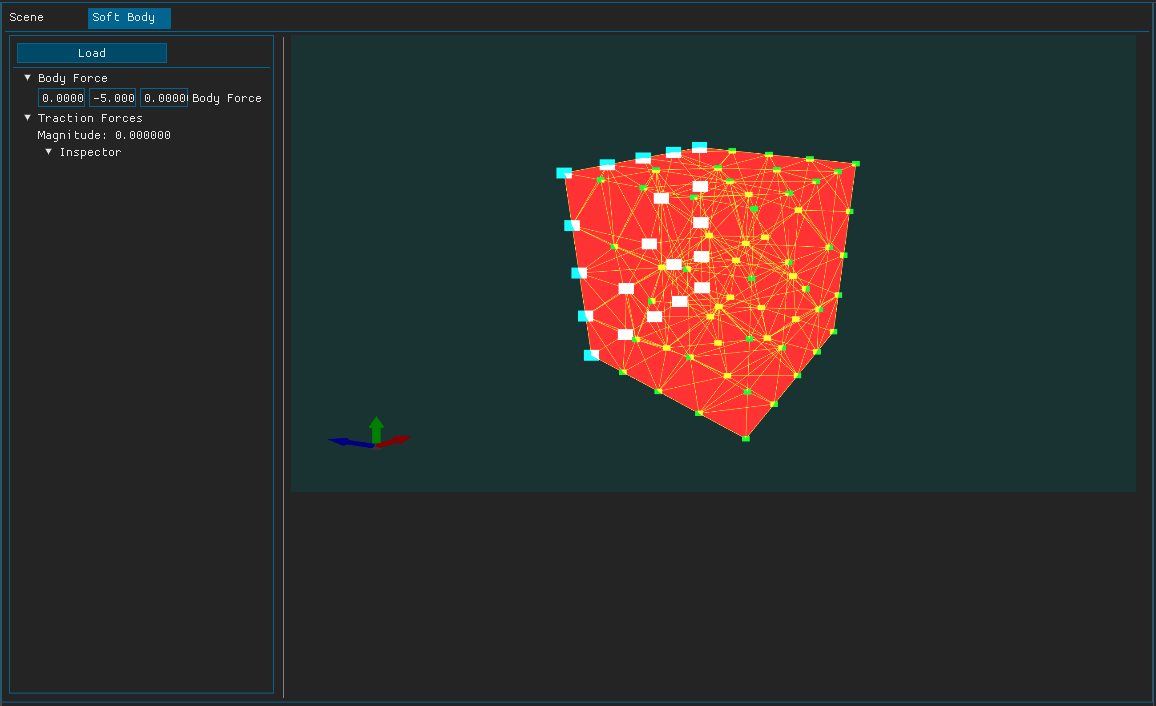
\includegraphics[scale=0.3]{pictures/ifx/ifx_load.png}
\caption[Soft body editor. Load panel]{Soft body editor. Load panel}
\label{fig:ifx_load}
\end{figure}

Finally, the solver panel is shown in figure~\ref{fig:ifx_solver1}. Build button assembles the model using the geometry and parameters chosen in previous panels. Play button starts the simulation. Step button steps the simulation by a single iteration. We can choose the frequency of physics simulation and the synchronization of output displacements with vertex buffer object. Time restrictions can be selected to stop the simulation after input amount of seconds. We can select if the solver should be computed on GPU or CPU. Linear solver can be chosen between Conjugate Gradient and LU decomposition. Figure~\ref{fig:ifx_solver2} shows the same model after about 20 seconds of simulation. The cube has been deformed under the gravity force. The timers are uses to profile the solver algorithms. It shows the time of computations for the last iteration.

\begin{figure}[h!]
\centering
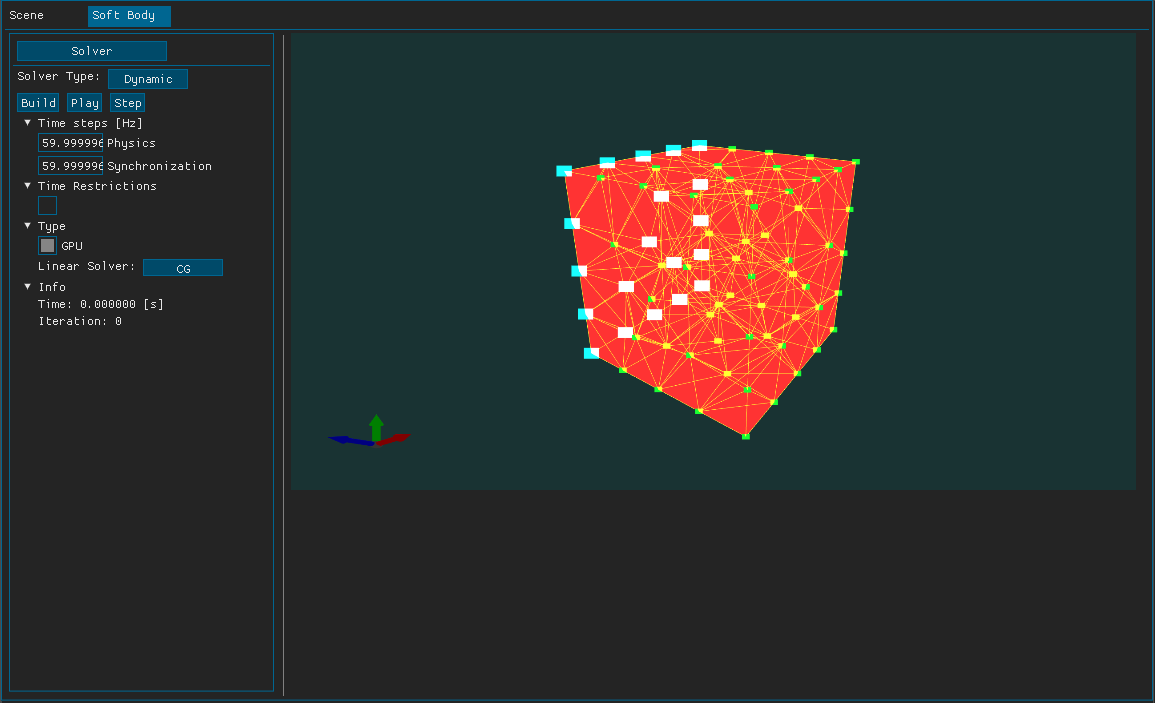
\includegraphics[scale=0.3]{pictures/ifx/ifx_solver1.png}
\caption[Soft body editor. Solver panel]{Soft body editor. Solver panel}
\label{fig:ifx_solver1}
\end{figure}

\begin{figure}[h!]
\centering
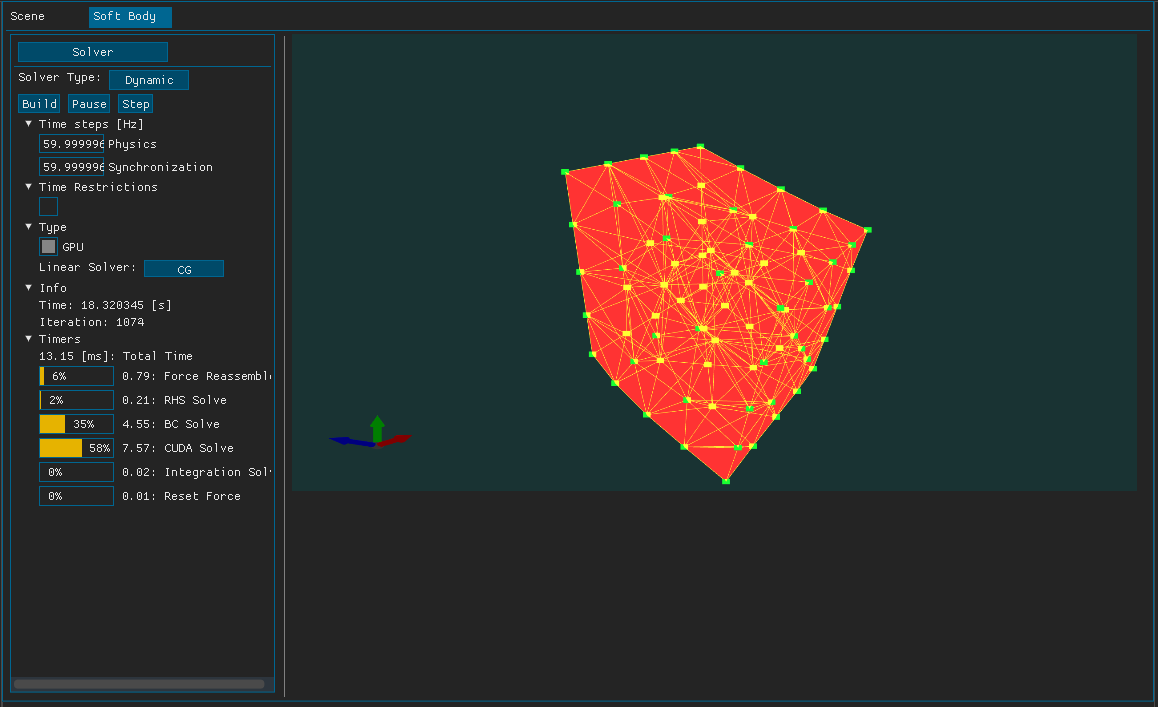
\includegraphics[scale=0.3]{pictures/ifx/ifx_solver2.png}
\caption[Soft body editor. Solver panel during computations]{Soft body editor. Solver panel during computations}
\label{fig:ifx_solver2}
\end{figure}

% ---------------------------------------------------

\chapter{Tests}
\label{chap:tests}


\chapter{Conclusions}
\label{chap:Conclusions}

The proposed real-time FEM solver library has been integrated into existing game engine. The library runs in parallel with existing physics and graphical modules. The two modules are fully decoupled and communicate only through a common game modules. Such architecture supports cheaper maintenance of entire system and makes it easy to inject other  soft body libraries.
The high level abstraction of the library reflects process of designing a FEM model. Thus, it was trivial to create a visual editor in which the user can design and solve FEM models.
GPU solver has obviously been proven to run much faster than a CPU for a large enough vertex count.

\section{Further work}

The two most expensive procedures of solver iteration include computing the right hand side vector and solving linear system of equations. Those procedures have been fully accelerated on the GPU. Other procedures such as applying boundary conditions or computing the force vector are now causing bottleneck due to their CPU implementation. Further work should look into accelerating these procedures on the GPU side as well.

Soft body deformation based on FEM formulation can support fracture mechanism. Stress magnitude can be calculated at each vertex. After overcoming a certain yield threshold the material would start breaking.

The proposed algorithm used a linear formulation of solid mechanics. This can only model small deformations. Next step of research should include study of GPU accelerated non-linear solvers. Such solvers could implement more accurate formulation for solid mechanics. Moreover, the solver could also include solutions for heat transfer problems and the coupling between the thermal and solid mechanics. Such solution would improve accuracy and provide even more realism to virtual environments.

It would be interesting to see how the proposed soft body solution checks out with virtual reality hardware. The user would be able to deform a body by applying pressure using their hand controller. Moreover, soft body could be grabbed by any of the boundary vertices. Such a user interface could be a great realism test.


% 6. Bibliografia
% Bibliografia leksykograficznie wg nazwisk autorów

\begin{thebibliography}{20}%jak ktoś ma więcej książek, to niech wpisze większą liczbę
% \bibitem[numerek]{referencja} Autor, \emph{Tytuł}, Wydawnictwo, rok, strony
% cytowanie: \cite{referencja1, referencja 2,...}

% FEM Books

\bibitem[1]{termo} Michał Kleiber, Piotr Kowalczyk, \emph{Wprowadzenie do Nieliniowej Termomechaniki Ciał Odkształcalnych}.

\bibitem[2]{zienkiewicz1} Zienkiewicz \emph{The Finite Element Method. Volume 1: The Basis}.

\bibitem[3]{zienkiewicz2} Zienkiewicz \emph{The Finite Element Method. Volume 2: Solid Mechanics}.

\bibitem[4]{altair} Altair University \emph{Practical Aspects of Finite Element Simulation}.

\bibitem[5]{colorado_fem_lectures} Department of Aerospace Engineering Sciences University of Colorado at Boulder \emph{Advanced Finite Element Methods (ASEN 6367) Lectures https://www.colorado.edu/engineering/CAS/courses.d/AFEM.d/}.

% Notes

\bibitem[6]{physics_notes} Matthias Muller, Jos Stam, Doug James, Nils Thurey, \emph{Real Time Physics Class Notes}.

\bibitem[7]{cg} Jonathan Richard Shewchuk \emph{An Introduction to the Conjugate Gradient Method Without the Agonizing Pain}.

\bibitem[8]{delaunay_mesh} Jonathan Richard Shewchuk \emph{Lecture Notes on Delaunay Mesh Generation}.

\bibitem[9]{tetgen} Hang Si \emph{A Quality Tetrahedral Mesh Generator and 3D Delaunay Triangulator}.

% FEM Papers

\bibitem[10]{flex} Miles Macklin, Matthias Muller, Nuttapong Chentanez, Tae-Yong Kim \emph{Unified Particle Physics for Real-Time Applications}.

\bibitem[11]{parker} Eric G. Parker, James F. O'Brien \emph{Real-Time Deformation and Fracture in a Game Environment}.

\bibitem[12]{tensor-mass} X. Faure, F. Zara, F. Jaillet, J-M. Moreau  \emph{An implicit Tensor-Mass solver on the GPU for soft bodies simulation}.

\bibitem[13]{global_deformation} Yan Zhuang, John Canny \emph{Real-time Simulation of Physically Realistic Global Deformation}.

% Third party software

\bibitem[14]{bullet} Bullet \emph{http://www.bulletphysics.org/mediawiki-1.5.8/index.php/Documentation}.

\bibitem[15]{opengl} OpenGl \emph{https://www.opengl.org/}.

\bibitem[16]{sofa} SOFA Framework \emph{https://www.sofa-framework.org}.

\bibitem[17]{physx} NVIDIA \emph{http://docs.nvidia.com/gameworks/content/gameworkslibrary/physx/guide/Manual/Index.html}.

\bibitem[18]{cublas} NVIDIA cuBLAS \emph{http://docs.nvidia.com/cuda/cublas/index.html}.

\bibitem[19]{cusparse} NVIDIA cuSPARSE \emph{http://docs.nvidia.com/cuda/cusparse/index.html}.

\bibitem[20]{eigen} Eigen \emph{http://eigen.tuxfamily.org/index.php?title=Main\_Page}.

\bibitem[21]{googletest} Google \emph{https://github.com/google/googletest}.

% Source codes

\bibitem[22]{ifx} Jakub Ciecierski \emph{https://github.com/Jakub-Ciecierski/InfinityXLib}.

\bibitem[23]{rtfem} Jakub Ciecierski \emph{https://github.com/Jakub-Ciecierski/RT-FEM}.

\bibitem[24]{JC-MassSpring} Jakub Ciecierski, \emph{https://github.com/Jakub-Ciecierski/SoftBodySimulation}


\end{thebibliography}

% 7. Wykaz symboli i skrótów - jeśli nie ma, zakomentować
\chapter*{Wykaz symboli i skrótów}

\begin{tabular}{cl}
FEM & Finite Element Method \\
GPU & Graphics Processing Unit \\
CPU & Central Processing Unit \\
PDE & Partial Differential Equation \\
ODE & Ordinary Differential Equation \\
\end{tabular}


% 8. Spis rysunków - jeśli nie ma, zakomentować (ale być może po prostu się nie zrobi)
\listoffigures


% 9. Spis tabel - jak wyżej
\renewcommand{\listtablename}{Spis tabel}
\listoftables


% 10. Spis załączników - jak nie ma załączników, to zakomentować lub usunąć

%\chapter*{Spis załączników}
%\begin{enumerate}
%\item[1.] Załącznik 1
%\item[2.] Załącznik 2
%\end{enumerate}

% 11. Załączniki
%\newpage
%\pagestyle{empty}
%Załącznik 1, załącznik 2 -- mają się znajdować na końcu pracy (to jest notka przypominająca)

\end{document}

